% options:
% thesis=B bachelor's thesis
% thesis=M master's thesis
% czech thesis in Czech language
% slovak thesis in Slovak language
% english thesis in English language
% hidelinks remove colour boxes around hyperlinks

\documentclass[thesis=M,czech]{FITthesis}[2012/06/26]

\usepackage[utf8]{inputenc} % LaTeX source encoded as UTF-8

\usepackage{graphicx} %graphics files inclusion
% \usepackage{amsmath} %advanced maths
% \usepackage{amssymb} %additional math symbols

\usepackage{dirtree} %directory tree visualisation

% % list of acronyms
% \usepackage[acronym,nonumberlist,toc,numberedsection=autolabel]{glossaries}
% \iflanguage{czech}{\renewcommand*{\acronymname}{Seznam pou{\v z}it{\' y}ch zkratek}}{}
% \makeglossaries

\newcommand{\tg}{\mathop{\mathrm{tg}}} %cesky tangens
\newcommand{\cotg}{\mathop{\mathrm{cotg}}} %cesky cotangens

% % % % % % % % % % % % % % % % % % % % % % % % % % % % % % 
% ODTUD DAL VSE ZMENTE
% % % % % % % % % % % % % % % % % % % % % % % % % % % % % % 

\department{Katedra teoretické informatiky}
\title{Aplikace pro analýzu textových zpráv pro potřeby vyšetřovatelů}
\authorGN{Štěpán} %(křestní) jméno (jména) autora
\authorFN{Škorpil} %příjmení autora
\authorWithDegrees{Bc.~Štěpán Škorpil} %jméno autora včetně současných akademických titulů
\supervisor{Ing.~Pavel Kordík, Ph.D.}
\acknowledgements{Chtěl bych poděkovat všem, kteří mě podporovali během tvorby diplomové práce, ale i~během celého studia. Děkuji především celé rodině, všem přátelům a~zvlášť své přítelkyni za trpělivost, které se mi dostávalo.}
\abstractCS{Cílem této práce je navrhnout a~implementovat software pro zpracování textových dokumentů v~českém jazyce, který by mohla Policie České republiky využít v~boji se zločinem.

Výsledkem práce je první část komplexního řešení, která se zabývá prohledáváním dokumentů, automatickým tříděním do shluků a~hledáním podobných dokumentů. Práce se snaží dosáhnout cílů hledáním vhodných algoritmů pro stemizaci českého textu.}
\abstractEN{Sem doplňte ekvivalent abstraktu Vaší práce v~angličtině.}
\placeForDeclarationOfAuthenticity{V~Praze}
\declarationOfAuthenticityOption{4} %volba Prohlášení (číslo 1-6)
\keywordsCS{Vyhledávání, Indexace, Stemizace českého textu, Shluková analýza}
\keywordsEN{Searching, Indexing, Stemming of Czech text, Cluster analysis}

\begin{document}

% \newacronym{CVUT}{{\v C}VUT}{{\v C}esk{\' e} vysok{\' e} u{\v c}en{\' i} technick{\' e} v~Praze}
% \newacronym{FIT}{FIT}{Fakulta informa{\v c}n{\' i}ch technologi{\' i}}


\begin{introduction}
Policie České republiky uchovává velké množství dokumentů. Jedná se o výpovědi, oznámení a~stručné zprávy týkající se různých případů v~čistě textové podobě, bez jakékoliv pevné struktury či atributů, psané v~českém spisovném jazyce. Z~těchto dokumentů je potřeba seskládat či vytěžit jakékoliv užitečné informace, které by vedly k~dopadení pachatelů.

Nástrojů v~oblasti získávání různých druhů dat z~textu a~jejich vizualizace existuje celá řada, mezi nejpoužívanější patří Rapid Miner, R či GATE. Tyto programy většinou disponují nástroji pro zpracování anglického textu, popřípadě pro zpracování textu v jiném světovém jazyce. Horší je situace s~nástroji pro zpracování dokumentů v~českém jazyce. Existuje několik komerčních řešení, avšak žádný jednoduše použitelný open source program.

Z těchto důvodů se zadavatel práce obrátil s~problémem na Fakultu informačních technologií ČVUT. Na následujících stránkách této práce se pokusím navrhnout a~implementovat nástroje pro zpracování českého textu a~aplikaci, která pomůže vyšetřovatelům v~jejich práci.
\end{introduction}
\chapter{Analýza}
\label{analysis}
\section{Analýza požadavků}
V~první řadě jsem musel zjistit, co vyšetřovatelé od nové aplikace očekávají. Po konzultaci se zadavatelem práce jsem zjistil následující. 

Policie uchovává data jako RTF dokumenty v~MSSQL databázi. Zadavatel je schopen exportovat tyto dokumenty do plain textových souborů. Právě takto získané soubory chce zpracovávat. Vstupem pro software tedy bude jeden či více adresářů v~souborovém systému s textové soubory.

Soubory jsou čistě textové, bez jakékoliv pevné struktury či atributů, psané v~přirozeném spisovném českém jazyce. Soudě podle anonymizovaných příkladů, které mi byly poskytnuty, jsou to výpovědi, oznámení, stručné zprávy a~další úřední záznamy týkající se různých případů.

Aplikace by měla při indexaci vnitřně uchovat celý obsah dokumentu, protože zadavatel počítá s~tím, že po zaindexování exportované soubory smaže ze souborového systému počítače.

První požadavek se týká vyhledávání. V~souborech je potřeba najít ty texty, které se týkají daného tématu nebo případu. Bude tedy nutné nasadit či vytvořit fulltextový vyhledávací nástroj, který bude umět indexovat zdrojové texty v~adresářové struktuře a~poté texty vyhledat pomocí dostatečně robustního dotazovacího jazyka. Nástroj bude muset zvládnout provádět nad českými zdrojovými texty základní operace pro vytěžování dat, tj. tokenizaci a~lematizaci nebo stemizaci.

Ve výsledcích hledání by měla být zvýrazněna hledaná slova. Dále by výsledky hledání mělo být možné automaticky seskupit podle shlukové analýzy. Systém by měl být také schopen nabídnout podobné dokumenty k~již otevřenému dokumentu.

Dále je třeba ze souborů získat ryzí informace. V~první řadě by nástroj měl umět extrahovat z~textu entity, kterých se text týká. Tyto entity by pak měly být také indexovány aby podle nich mohly být texty vyhledány. K~vyhledání entit v~textu bude zapotřebí dalších, složitějších nástrojů pro zpracování textu. Bude k~tomu nezbytné zjistit slovní druh jednotlivých slov a~také vytvořit či získat rozsáhlé slovníky jmenných entit. 

Nejnáročnější funkcí, kterou by software v~tomto prostředí měl zvládat, je extrakce souvislostí a~vztahů mezi entitami.

Zadavatel požaduje, aby byla aplikace postavena na klient-server architektuře. Složky s~dokumenty totiž budou umístěny na jediném počítači a~uživatelům by mělo být umožněno s~daty pracovat na svých počítačích v~síti nezávisle na sobě. Usoudil jsem, že nejlepší volbou bude vytvořit aplikaci webové rozhraní. Je to řešení moderní, které dostojí požadavku klient-server architektury a~zároveň s ním odpadá jakákoliv správa aplikace na klientských počítačích.

Aplikace bude nasazena na běžném stolním počítači s~operačním systémem Windows. Zadavatel se ale v~případě nutnosti nebrání nasazení aplikace ve virtualizovaném linuxovém stroji pod Windows.

Požadavky, které jsou na aplikaci kladeny, by se tedy daly shrnout do následujících bodů.

\subsection{Funkční požadavky}
\label{req_0}
\begin{enumerate}
	\item \label{req_00} Systém bude indexovat textové soubory přímo z~adresářové struktury počítače.
	\item \label{req_01} Systém bude umožňovat rozšíření o~další nezávislý index dokumentů.
	\item \label{req_02} Systém si bude ukládat celý obsah dokumentů.
	\item \label{req_03} Systém bude zpracovávat text v~české jazyce.
	\item \label{req_04} Systém bude umožňovat fulltextové vyhledávání v~indexovaných dokumentech.
	\begin{enumerate}
		\item \label{req_040} Systém bude k~tomuto účelu zvládat tokenizaci českého textu.
		\item \label{req_041} Systém bude k~tomuto účelu zvládat stemizaci českého textu.
		\item \label{req_042} Systém bude umožňovat zobrazit obsah nalezených dokumentů.
		\item \label{req_043} Systém bude zvýrazňovat hledaná slova ve výsledcích hledání.
	\end{enumerate}
	\item \label{req_05} Systém bude umožňovat zobrazení podobných dokumentů.
	\begin{enumerate}
		\item \label{req_050} Systém bude k~tomuto účelu vyhodnocovat podobnost dokumentů.
	\end{enumerate}
	\item \label{req_06} Systém bude umožňovat shlukovat výsledky hledání do automaticky generovaných kategorií.
	\begin{enumerate}
		\item \label{req_060} Systém bude k tomuto účelu provádět shlukovou analýzu.
		\item \label{req_061} Systém bude umožňovat filtrovat výsledky podle zvolených shluků.
	\end{enumerate}
	\item \label{req_07} Systém bude umožňovat rozpoznávat jmenné entity.
	\begin{enumerate}
		\item \label{req_070} Systém bude k~tomuto účelu umět rozpoznávat větné členy.
		\item \label{req_071} Systém bude k~tomuto účelu umět rozpoznávat slovní druhy.
		\item \label{req_072} Systém bude k~tomuto účelu obsahovat jmenné databáze.
	\end{enumerate}
	\item \label{req_08} Systém bude umožňovat extrakci vazeb mezi entitami.
\end{enumerate}

\subsection{Nefunkční požadavky}
\label{req_1}
\begin{enumerate}
	\item \label{req_10} Systém bude postaven pouze na open source technologiích.
	\item \label{req_11} Systém bude postaven na architektuře klient-server jako webová služba.
	\item \label{req_12} Systém bude nativně nasaditelný pod operačním systémem Windows (není podmínkou).
	\item \label{req_13} Systém bude rozšiřitelný.
\end{enumerate}

\subsection{Stanovení první fáze}
Definované požadavky jsou velmi rozsáhlé a~z~části na sebe navazují svými vstupy a~výstupy. Je tedy potřeba začít od základních požadavků a~ty pak rozšiřovat o~další možnosti zpracování. Celý definovaný rozsah je nad rámec jedné diplomové práce a~tak bylo potřeba projekt rozčlenit do několika fází.

První fáze sestává z~tvorby vyhledávání v~textu, a~to z~toho důvodu, že je jakýmsi základem dalších operací s~textem. Pro fulltextové vyhledávání musí text projít tokenizací, stemizací a~následně indexací do databáze. Na produkty těchto základních operací další operace navazují.

Do první fáze projektu jsem pak ještě doplnil o shlukovou analýzu výsledků vyhledávání a~výpočet podobnosti dokumentů, protože s vyhledáváním úzce souvisí.

Další části této práce se už budou zabývat jen první fází projektu. V návrhu aplikace pak budu brát na zřetel budoucí možnost rozšíření o~další definované požadavky.

\section{Aktéři systému}
Z~definovaných požadavků vzešli aktéři a~případy užití systému. Obojí je názorně zobrazeno v~diagramu \ref{fig:UseCases}. V systému budou figurovat prakticky jen dvě uživatelské role a~jeden neuživatelský aktér, systémový plánovač.

\begin{enumerate}
	\item \label{itm:actor_user}Uživatel: Aktér, který bude systém používat pro získávání informací z~textu. Všechny scénáře tohoto aktéra mají jako prerekvizitu index již naplněný dokumenty k prohledávání.
	\item \label{itm:actor_admin}Správce: Aktér bude moci provádět vše co uživatel, jen navíc bude spravovat index dokumentů. Aktér bude mít plný přístup k~serverovému stroji.
	\item \label{itm:actor_scheduler}Systémový plánovač: Některé scénáře mohou být plánovány a~spouštěny automaticky systémem. Jsou řízeny nastaveným časem.
\end{enumerate}

\begin{figure}[h]
\begin{center}
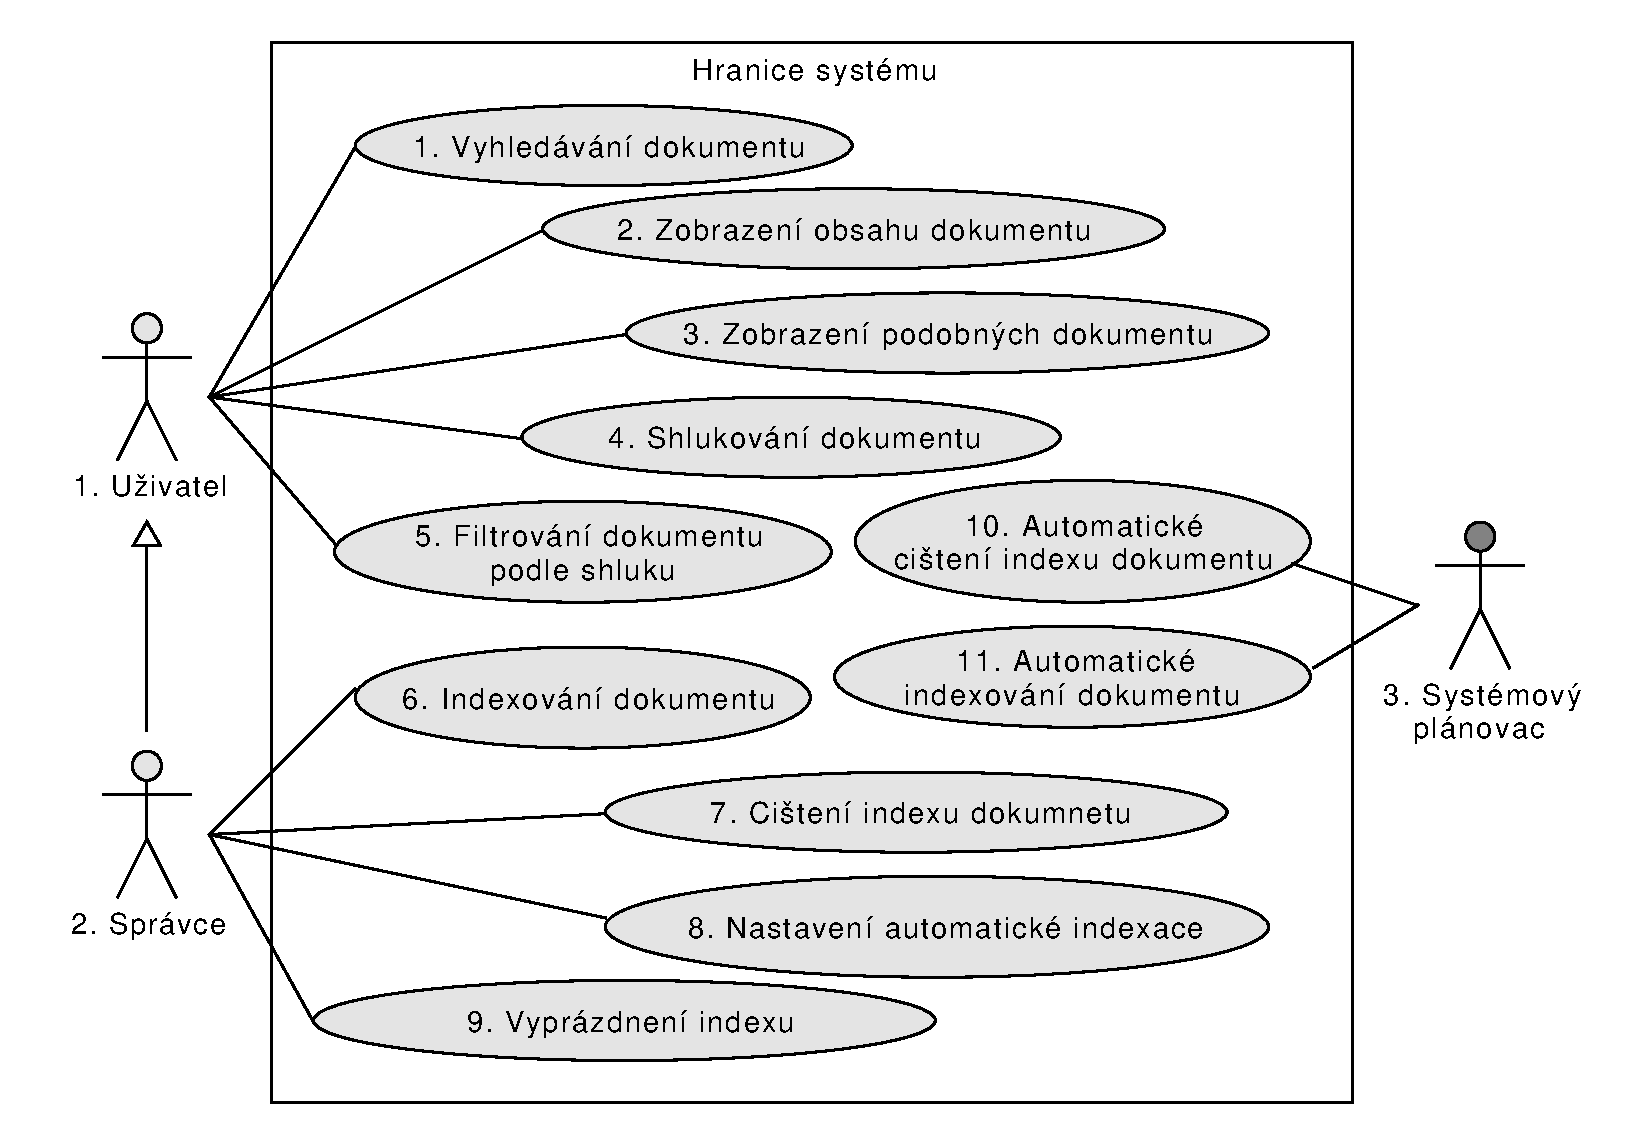
\includegraphics[width=13cm]{UseCases}
\caption{Diagram případů užití}
\label{fig:UseCases}
\end{center}
\end{figure}

\section{Případy užití}

\subsection{Vyhledávání dokumentů}
\begin{itemize}
	\item[Aktéři] \ref{itm:actor_user} Uživatel
	\item[Scénář:]
	\begin{enumerate}
		\item Uživatel zadá dotaz.
		\item Systém zobrazí výsledky dle dotazu.
	\end{enumerate}
	\item[Výstup:] Dokumenty odpovídající dotazu
\end{itemize}

\subsection{Zobrazení obsahu dokumentů}
\begin{itemize}
	\item[Aktéři:] \ref{itm:actor_user} Uživatel
	\item[Scénář:]
	\begin{enumerate}
		\item Uživatel zvolí zdroj a~zadá dotaz.
		\item Systém zobrazí výsledky dle dotazu.
		\item Uživatel ze zobrazených výsledků vybere požadovaný dokument.
		\item Systém zobrazí obsah dokumentu.
	\end{enumerate}
	\item[Výstup:] Zobrazený obsah dokumentu
\end{itemize}

\subsection{Zobrazení podobných dokumentů}
\begin{itemize}
	\item[Aktéři:] \ref{itm:actor_user} Uživatel
	\item[Scénář:]
	\begin{enumerate}
		\item Uživatel zvolí zdroj a~zadá dotaz.
		\item Systém zobrazí výsledky dle dotazu.
		\item Uživatel ze zobrazených výsledků vybere požadovaný dokument.
		\item Systém zobrazí seznam dalších dokumentů seřazených od nejpodobnějšího k nejméně podobnému
	\end{enumerate}
	\item[Výstup:] Dokumenty, které jsou podobné zvolenému dokumentu, seřazené od nejpodobnějšího k nejméně podobnému
\end{itemize}

\subsection{Shlukování dokumentů}
\begin{itemize}
	\item[Aktéři:] \ref{itm:actor_user} Uživatel
	\item[Scénář:]
	\begin{enumerate}
		\item Uživatel zvolí zdroj a~zadá dotaz.
		\item Systém zobrazí jak výsledky dle dotazu, tak nalezené shluky výsledných dokumentů.
	\end{enumerate}
	\item[Výstup:] Seznam shluků výsledných dokumentů
\end{itemize}

\subsection{Filtrování dokumentů podle shluků}
\begin{itemize}
	\item[Aktéři:] \ref{itm:actor_user} Uživatel
	\item[Scénář:]
	\begin{enumerate}
		\item Uživatel zvolí zdroj a~zadá dotaz.
		\item Systém zobrazí výsledky dle dotazu a~nalezené shluky výsledných dokumentů.
		\item Uživatel vybere jeden či více shluků.
		\item Systém zobrazí jen dokumenty patřící do zvolených shluků.
	\end{enumerate}
	\item[Výstup:] Seznam dokumentů v~daných shlucích.
\end{itemize}

\subsection{Indexování dokumentů}
\label{subsec:usecase_index}
\begin{itemize}
	\item[Aktéři:] \ref{itm:actor_admin} Správce
	\item[Scénář:]
	\begin{enumerate}
		\item Správce zvolí jeden či více adresářů.
		\item Systém v~adresářích najde textové soubory a~přidá je do indexu.\label{itm:scenary_index}
	\end{enumerate}
	\item[Výstup:] Zaindexované soubory ze zvolených adresářů připravené pro vyhledávání
\end{itemize}

\subsection{Čištění indexu dokumentů}
\label{subsec:usecase_clean}
\begin{itemize}
	\item[Aktéři:] \ref{itm:actor_admin} Správce
	\item[Scénář:]
	\begin{enumerate}
		\item Správce spustí čištění indexu.
		\item Systém projde dokumenty a~ty, které již neexistují v~souborovém systému, odstraní z~indexu.\label{itm:scenary_clean}
	\end{enumerate}
	\item[Výstup:] Index obsahující pouze dokumenty, které mají svou reprezentaci v~souborovém systému počítače
\end{itemize}

\subsection{Vyprázdnění indexu}
\begin{itemize}
	\item[Aktéři:] \ref{itm:actor_admin} Správce
	\item[Scénář:]
	\begin{enumerate}
		\item Správce spustí vyprázdnění indexu.
		\item Systém odstraní všechny dokumenty z~indexu.
	\end{enumerate}
	\item[Výstup:] Prázdný index
\end{itemize}

\subsection{Nastavení automatické indexace}
\begin{itemize}
	\item[Aktéři:] \ref{itm:actor_admin} Správce
	\item[Scénář:]
	\begin{enumerate}
		\item Správce zvolí interval, adresáře, zda se má indexovat, zda se má čistit index.
		\item Systém ve zvolený čas spouští čištění a~indexaci, viz aktér \ref{itm:actor_scheduler}  Systémový plánovač.
	\end{enumerate}
	\item[Výstup:] Nastavený systémový plánovač
\end{itemize}

\subsection{Automatické indexování dokumentů}
\begin{itemize}
	\item[Aktéři:] \ref{itm:actor_scheduler} Systémový plánovač
	\item[Scénář:]
	\begin{enumerate}
		\item Plánovač nastaví konfiguraci dle nastavení uživatele.
		\item Systém pokračuje v~indexaci od bodu \ref{itm:scenary_index} scénáře \ref{subsec:usecase_index} Indexování dokumentů.
	\end{enumerate}
\end{itemize}

\subsection{Automatické čištění indexu dokumentů}
\begin{itemize}
	\item[Aktéři:] \ref{itm:actor_scheduler} Systémový plánovač
	\item[Scénář:]
	\begin{enumerate}
		\item Plánovač nastaví konfiguraci dle nastavení uživatele.
		\item Systém pokračuje v~indexaci od bodu \ref{itm:scenary_clean} scénáře \ref{subsec:usecase_clean} Čištění indexu dokumentů.
	\end{enumerate}
\end{itemize}

\section{Technologie}
\subsection{Surmon}
Bylo mi navrženo, abych se pokusil implementovat práci pomocí nástroje Surmon. Prostudoval jsem si tedy  dokumentaci aplikace, otestoval si její funkce a~zjistil následující.

Surmon je balík modulů pro platformu OBBB\cite{surmon:guide} — Open Black Box Builder. Platforma OBBB umožňuje sestavit aplikaci pro zpracování dat pomocí propojování funkčních bloků. Blok je atomický kus algoritmu se vstupy a~výstupy různých datových typů a~s~možností nastavení parametrů pro úpravu jeho chování. Každý blok načte data na svých vstupech, zpracuje je a~výsledná data zapíše na své výstupy. Bloky pak lze propojovat spojnicemi z~výstupu jednoho bloku na vstup jiného — samozřejmě jen tehdy, jsou–li kompatibilní datové typy vstupů a~výstupů.  Takovouto tvorbou orientovaných grafů bloků a~spojnic lze definovat složité algoritmy. Na sestavování bloků má platforma již vytvořený intuitivní editor v~podobě plátna, na které se bloky přidávají a~kde se propojují. Každý blok má svou reprezentaci v~uživatelském rozhraní, pomocí kterého lze nastavit parametry bloku. Vše je implementováno v~jazyce Java a~postaveno na Platformě NetBeans\cite{netbeans:guide}.

Samotný OBBB obsahuje základní sadu bloků pro řízení toku algoritmu, načítání a~zápis souborů různých formátů, iteraci nad daty a~další funkce. Surmon je pak sada dalších bloků pro operace zpracování textu a~text mining. Pro účely této práce je podstatné zejména to, že Surmon obsahuje bloky pro text mining z českých textů.

Software tedy umožňuje sestavit algoritmy pomocí hotových celků bez programátorského zásahu. Sestavený alogritmus pak lze uzamknout heslem, vystavit některé vstupy či parametry nastavení jako uživatelské rozhraní a~nabízet vzniklou aplikaci jako hotové řešení.

Platforma umožňuje poměrně snadnou tvorbu nových bloků. Má k~tomu velmi detailně definované a~dokumentované rozhraní. Lze tedy vytvořit bloky pro další dílčí práci s~daty, které následně lze použít stejným způsobem jako bloky vestavěné.

Software Surmon mě velice zaujal, ale pro tuto práci jsem jej nakonec nevyužil. Hlavní problém je v~požadavku klient-server architektury. Zkoumal jsem možnosti rozšířit software pomocí nových bloků tak, aby šel použít i~v~klient-server architektuře, aby například blok začal poslouchat na síťovém portu na příchozí dotazy, nebo aby jen předzpracovával data do indexu přičemž jiná aplikace by dodávala na základě tohoto indexu výsledky na vyhledávací dotazy. Všechny takové možnosti jsou příliš těžkopádné. Bloky jsou navrhovány jen na přijetí dat, zpracování a~odeslání dat dál v~řetězci. Vstupní  jsou v~programu všechny bloky které nemají vlastní vstupy. Bloky se pak postupně zpracovávají v~samostatných vláknech. Při takovém návrhu není snadné zařídit poslouchání na síťovém portu a~odpovídání na požadavky.

Jinými slovy, Surmon je stavěn k ověřování konceptů různých algoritmů, nebo k~tvorbě jednoúčelového text miningového softwaru jako tzv. standalone aplikace na jednom počítači. Nehodí se na finální řešení k~poskytování síťových služeb.

Kromě toho, aby mi byl software poskytnut pro implementaci projektu, muselo by být celé textové zpracování implementováno v~Surmonu. Tvůrci Surmonu se totiž snaží bránit jakémukoliv vyvádění implementovaných knihoven ven ze softwaru. Mimo Surmon tedy nleze implementované knihovny využít.

\subsection{Solr}
Protože nástroj Surmon nelze pro můj projekt použít, začal jsem hledat open source software, který by pomohl s~fulltextovým vyhledáváním, byl rozšiřitelný a~ zároveň by šel zakomponovat do složitější architektury. Objevil jsem Solr\cite{sorl:wiki}, platformu pro fulltextové vyhledávání vyvíjenou pod licencí Apache License nadací Apache Software Foundation ve spolupráci s~projektem Lucene. 

Solr je napsaný v~jazyce Java, který mu  zajišťuje multiplatformnost, takže může fungovat i~pod systémem Windows, který je zadavatelem preferován.

Solr je vlastně vyhledávací server běžící v~servlet containerech, jako jsou Jetty či Apache Tomcat. Poskytuje REST rozhraní  pro integraci s~jinými aplikacemi v~různých jazycích. Solr v~základní instalaci podporuje hned několik datových formátů pro REST komunikaci, například JSON a~XML. Kromě REST rozhraní jsou k~dispozici již hotové knihovny pro mnoho programovacích jazyků, které ještě více pomohou integrovat Solr s~dalšími aplikacemi. Příkladem je Javová knihovna \emph{SolrJ}, nebo JavaScriptové knihovny \emph{AJAX Solr} nebo \emph{Solr Search}.

Jako fulltextové vyhledávací jádro používá Solr knihovnu Lucene, jejíž funkce zprostředkovává pro samostatné serverové použití. Knihovna Lucene je také napsaná v~jazyce Java, existují však i~její portace do jiných jazyků. Knihovna slouží pro tvorbu a~správu indexu a~následné vyhledávání v~indexu. Na svých stránkách\cite{lucene:wiki} se tvůrci chlubí nízkou náročností na hardware počítače, širokou podporou různých způsobů dotazování, podporou simultálního aktualizace indexu a~vyhledávání, podporou spojování výsledků z~různých indexů a~dalších pokročilých funkcí.

Solr sbírá (indexuje) a~prohledává (dotazuje) index dokumentů. Dokument je pro Solr jednotka informace. Sestává z~atributů, polí daného datového typu, anglicky fields.  Z~jakých polí se dokument skládá charakterizuje tzv. schéma. To lze nastavit v~konfiguračním souboru \emph{schema.xml}. Všechny dokumenty mají stejnou strukturu polí danou schématem. Schéma určuje i to, jakým způsobem mají být pole interpretována, zpracovávána a~dotazována. Tento proces tvůrci nazývají Field Analysis — analýza polí. Zde lze například nastavit, jaký tokenizer, stemmer, či filtr se má použít na dané pole. Tyto analyzéry jsou ničím jiným než Java třídami implementující dané rozhraní. Poměrně jednoduše lze tedy vytvořit jakýkoliv vlastní analyzér, který předzpracuje text v~poli.

Solr umožňuje použít k~jednomu poli jeden tokenizer, tj. prvek, který text rozdělí na jednotlivé indexované úseky — nejčastěji slova. Dále můžeme přiřadit 0–n char filterů, které očistí text od nepotřebných znaků, jako jsou HTML značky, a~0–n filtrů, které odstraní z~výstupu celá nechtěná slova. Na úryvku xml kódu můžeme pozorovat definice typu pole s~analyzéry zvlášť pro proces indexace a~pro dotazování a~přiřazení tohoto typu pole. V~ukázce si také můžeme všimnout nastavení pole indexed a~stored. To znamená, že se pole má indexovat a~zároveň se má v~databázi uchovat i~jeho původní plné znění, což je užitečné, jelikož podle indexu se rychle vyhledá daný dokument a~pak se může pole zobrazit ve výsledcích v~plném rozsahu.

V~konfiguraci pole lze povolit i~ukládání vektoru termů. Vektor lze potom využít pro další zpracování textu i~mimo samotný solr v~dalších fázích projektu.

Dalšími důležitými nastaveními v~schema.xml jsou: které pole bude unikátní identifikátor dokumentu, ve kterém poli se bude ve výchozím stavu vyhledávat, jaká třída bude vyhodnocovat podobnost dokumentů. Analyzéry mívají ještě další možnosti nastavení.

\begin{verbatim}
<fieldType name="text_general" class="solr.TextField" 
			  positionIncrementGap="100">
 <analyzer type="index">
   <tokenizer class="solr.StandardTokenizerFactory"/>
   <filter class="solr.StopFilterFactory" ignoreCase="true" 
 		     words="stopwords.txt" enablePositionIncrements="true" />
   <filter class="solr.SynonymFilterFactory" synonyms="index_synonyms.txt" 
           ignoreCase="true" expand="false"/>
   <filter class="solr.LowerCaseFilterFactory"/>
 </analyzer>
 <analyzer type="query">
   <tokenizer class="solr.StandardTokenizerFactory"/>
   <filter class="solr.StopFilterFactory" ignoreCase="true" 
           words="stopwords.txt" enablePositionIncrements="true" />
   <filter class="solr.SynonymFilterFactory" synonyms="synonyms.txt"
           ignoreCase="true" expand="true"/>
   <filter class="solr.LowerCaseFilterFactory"/>
 </analyzer>
</fieldType>

<field name="content" type="text_general" 
       indexed="true" stored="true" termVectors="true" />
\end{verbatim}

Zbývá se podívat na to, jak je na tom Solr s~podporou českého jazyka. Podle informací na oficiálních stránkách\cite{sorl:wiki} je Český jazyk nástrojem podporován již od verze 3.5. Lze prý použít standartní tokenizer \emph{StandardTokenizer}, který dělí text na tokeny nejen podle definovaných prázdných znaků, ale má sadu pravidel, která správně nechají v~celku zkratky, slova s~apostrofy a~podobně. K~tomu jsou doporučovány dva běžné filtry: \emph{LowerCaseFilter}, který převede token na malá písmena a~\emph{StopFilter}, který umožní definovat stop word list, seznam slov, která se mají vynechat z~indexu. Na závěr tvůrci doporučují pro český text použít \emph{CzechStemFilter}. Je to stemmer vycházející z~práce L.~Dolamica a~J.~Savoye, kteří se na Švýcarské University of Neuchatel zabývali stemizačními algoritmy východoevropských jazyků. Stemmer funguje s~tokeny již převedenými do malých písmen a~umí pracovat s~diakritikou. Funguje na principu postupného odebírání koncovek a~některých předpon slov.

Výsledky analýzy nástroje Solr lze tedy shrnout takto: Solr se zdá být vhodným kandidátem pro nasazení v~projektu. Neklade meze integraci s~jinými aplikacemi a~do jisté míry podporuje český jazyk. Nepochybně ale bude nutné otestovat kvalitu zpracování českých textů a~popřípadě nástroj rozšířit o~nové knihovny pro tento účel.

\subsection{Jetty}
Solr jako Java EE aplikace potřebuje servlet container ke svému běhu — Jetty. Jetty\cite{jetty:doc} je open source javový web server a~java servlet container, vyvíjený společností Eclipse Foundation. Pro projekt jsem zvažoval i~použití Apache Tomcat\cite{tomcat:doc}, se kterým už mám zkušenost z~předchozích projektů, ale narazil jsem na několik chyb a~nekompatibilit se Solrem. Zůstal jsem tedy nakonec u~Jetty, se kterým se Solr oficiálně distribuuje a~který oficiálně podporuje.

\subsection{Carrot2}
Jedním z~požadavků na projekt je shlukování výsledků vyhledávání. Zjistil jsem, že existuje javový open source shlukovací engine Carrot2\cite{carrot2:manual}, který má podporu v~jádře Solru. Engine je určený pro shlukování spíše menších kolekcí dat a hodí se tedy právě pro shlukování výsledků vyhledávání.

Carrot2 se distribuuje se třemi implementovanými algoritmy pro shlukování. Obsahuje algoritmus Bisekční K-means, který počítá vzdálenosti vektorů dokumentů nebo vektoru reprezentantů shluků a~vždy do shluku spojí 2 nejbližší sousedy až do požadovaného počtu shluků. Dále obsahuje algoritmus Lingo, který vytvořili S.~Osiński, J.~Stefanowski a D.~Weiss, založený na algebraických transformacích matic termů a~extrakci častých frází použitím sufixových polí. Posledním obsaženým algoritmem je STC, suffix tree clustering, který sestaví termy do sufixového stromu, aby nalezl prvotní zástupce shluků dokumentů.

Carrot2 obsahuje i~J2EE webovou aplikaci s~hotovým vyhledávacím rozhraním. Tato aplikace má možnost nakonfigurovat i~několik informačních zdrojů, ve kterých se bude vyhledávat. V~základu je několik zdrojů implementováno. Můžeme aplikaci napojit například na Wikipedii, Google, Bing i~Solr. Aplikace již podporuje zvýraznění hledaných slov ve výsledcích, zobrazení shluků i~filtrování dokumentů podle zvoleného shluku. Funguje tím způsobem, že dotaz přepošle na zdrojovou službu a~nad výsledky, které ji služba vrátí provede shlukovou analýzu. Následně pak zobrazí výsledky vyhledávání i~nalezené shluky. Shluky navíc umí zobrazit i~interaktivně v~grafické formě.

Carrot2 lze tedy k~Solru připojit dvěma způsoby. Jednou možností je nasadit Carrot2 jako samostatnou webovou aplikaci, která bude zprostředkovávat vyhledávací dotazy na Solr server a~výsledky vyhledávání před vrácením ještě podrobí shlukové analýze. V~tomto případě by ale musel Carrot2 být zároveň i~frontendem systému a~tak využiji druhé možnosti připojení: Carrot2 bude do Solru nainstalován a~nakonfigurován jako rozšiřující knihovna pro shlukování výsledků, která bude obohacovat výsledky vyhledávání o~výsledky shlukové analýzy. Tím se zachová možnost výběru frontendu.
\chapter{Návrh}
\section{Architektura} \label{arch}
V~této kapitole se pokusím navrhnout strukturu jednotlivých komponent výsledného řešení. Celá architektura systému je znázorněna na obrázku \ref{fig:Architecture}. Středobodem systému je server s~nainstalovaným servlet containerem Jetty. V~containeru bude nainstalován Solr. 

Solr bude tvořit backend aplikace. Bude do něj připojena knihovna \emph{Carrot2}, která rozšíří jeho možnosti o~shlukování výsledků, a~má vlastní knihovna s~implementovanými nástroji pro zpracování českého textu pojmenovaná \emph{Analyzery}. Solr bude tedy uchovávat index i~samotný obsah dokumentů, bude zpracovávat vyhledávací dotazy uživatelů a~vracet nalezené výsledky včetně informací o~shlucích a~o~podobnosti dokumentů.

Kromě Solru poběží v~Jetty ještě frontend aplikace. Frontend vytvořím vlastní tak, aby vyhovoval požadavkům. Solr tvoří solidní backend, který komunikuje pomocí HTTP rozhraní a~umožňuje vracet data ve snadno zpracovatelném JSON formátu. Rozhodl jsem se proto, že frontend bude tvořen několika statickými stránkami a~veškerá dynamika bude dodána pomocí JavaScriptu. Stránka se bude pomocí AJAX požadavků dotazovat přímo backendu aplikace --- Solru. Servlety tedy budou jen posílat statické HTML stránky, JavaScriptové knihovny, CSS styly a~podobné soubory. Výhoda řešení spočívá především v jeho jednoduchosti. Celý vyhledávací server bude fungovat v~jednom servlet containeru, vše se tedy zprovozní jen spuštěním nakonfigurovaného Jetty. Zároveň nebudu muset vytvářet stejné rozhraní dvakrát (jednou pro dotazování JavaScriptu webového serveru a~jednou pro dotazování webového serveru Solru).

Poslední komponentou v~architektuře je tzv. Crawler. To bude samostatná aplikace, jejímž úkolem bude indexovat soubory nebo naopak mazat chybějící soubory z~indexu. Připojovat se bude přímo na rozhraní Solru pomocí HTTP. Komunikace se Solrem bude síťová, díky čemuž může aplikace fungovat nejen na stejném stroji s~vyhledávacím serverem, ale i~na jakémkoliv počítači v~síti.

\begin{figure}[h]
\begin{center}
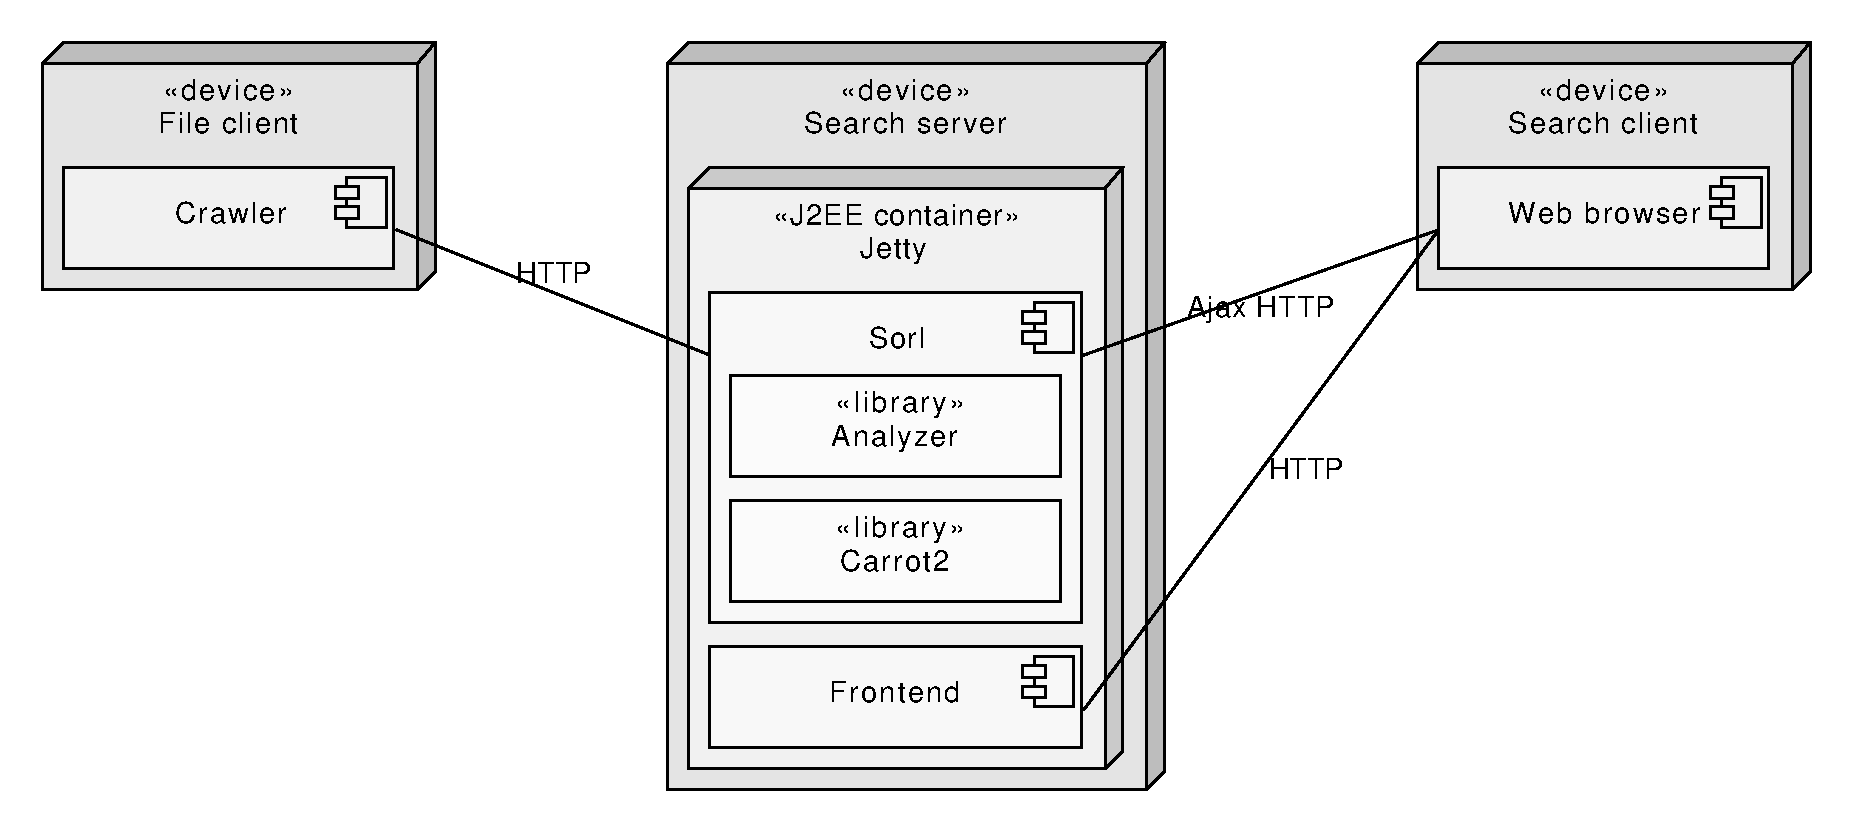
\includegraphics[width=13cm]{Architecture}
\caption{Diagram nasazení}
\label{fig:Architecture}
\end{center}
\end{figure}

\section{Crawler} \label{design_crawler}
Jedná se o~aplikaci, která dle nastavení projde rekurzivně složky file systému, vyhledá všechny soubory, sestaví z~nich Solr dokumenty a~pošle je k~indexaci do Solru. Dále bude procházet dokumenty v~Solru, kontrolovat, zda daný dokument ještě existuje ve filesystému, a~pokud ne, tak jej z~indexu odstraní. Jejím posledním úkolem je kompletní vyprázdnění indexu Solru.

Vzhledem k~tomu, že aplikace bude komunikovat se Solr serverem, rozhodl jsem se, že tuto aplikaci naprogramuji v~jazyce Java, jelikož pro Javu existuje oficiální Java knihovna \emph{Apache SolrJ} pro napojení na Solr server. Kromě této knihovny využiji ještě knihovnu \emph{Apache Log4J} pro zaznamenávání nastalých událostí, která je již závislostí \emph{SolrJ}, a~protože bude součástí aplikace, nebránil jsem se jejímu využití. Konfiguraci programu si usnadním využitím knihovny \emph{Apache commons-configuration}, která mi umožní definovat v~\emph{resources} adresáři výchozí konfigurační hodnoty, které ovšem bude možné přetížit hodnotami jinými pomocí externího konfiguračního souboru nebo pomocí argumentů programu. Díky tomu bude možné měnit chování programu podle aktuálních potřeb.

Aplikaci mám v~plánu navrhnout tak, aby byla rozšiřitelná o~další specializace výše sepsaných úkolů. Zadavetel totiž již během tvorby aplikace předložil několik nových návrhů k~jejímu rozšíření --- například aby aplikace podporovala načítání nejen textových souborů. Existuje také možnost (jak jsem psal v~kapitole \ref{analysis}), že v~budoucnu se bude aplikace napojovat přímo na databázi policejních dokumentů.

\subsection{Návrh tříd}
Během analýzy požadavků jsem nalezl několik společných rysů v~jednotlivých úkolech. Úkol vždy začíná procházením určitého média (např. indexu dokumentů či file systemu). Jednotlivé nalezené prvky (např. Solr dokumenty či soubory) se poté validují (kontroluje se existence na filesystému). V~dalším kroku se prvky parsují či konvertují do jiného datového formátu (soubor na Solr dokument), prvky se pak sbírají do kolekce a~jako kolekce se pak finálně zpracují (pošlou se na server k~zaindexování nebo se smažou z~indexu). Tyto shodné rysy jsem tedy postupně ještě více generalizoval, až jsem nakonec došel k~návrhu, který popisuji níže.

\subsubsection{Procesory}
Jednotlivé úkoly budou prováděny pomocí řetězce procesorů, tříd implementujících rozhraní \emph{IProcessor}.  Procesorové třídy jsou znázorněny v~diagramu \ref{fig:ProcessorClasses}. Řetězec vždy bude začínat \emph{Crawlerem}, tj. třídou, která prochází médium a~předává jednotlivé nalezené prvky prvnímu procesoru v~řetězci. Většina procesorů bude dědit od \emph{AbstractPassThroughProcessor}. Tyto procesory vždy vykonají určitou dílčí činnost a~produkt své činnosti pošlou dalšímu procesoru v~řetězci. Každý procesor bude mít jedinou funkci.

\emph{FactoryProcessor} bude konvertovat data z~jednoho formátu do druhého. Bude tak činit pomocí třídy implementující \emph{IFactory} rozhraní dle návrhového vzoru strategy. Implementovat budu dva typy těchto factory strategií. Jeden typ bude získávat \emph{SolrInputDokument} z~objektu \emph{File} (ten bude použit při indexování dokumentů). Vytvořím dvě implementace: jedna bude umět pouze načítat textové soubory, druhá bude určena pro načítání jakýchkoli textových dokumentů na disku za použití knihovny \emph{Tika}. Druhý typ factory strategie bude z~objektu \emph{SolrDocument} získávat id dokumentu pro kontrolu a~případné smazání z~indexu.

\emph{FilterProcessor} dokáže ze~vstupních dat odfiltrovat některé prvky tím, že je nepředá na výstup. Strategie filtrování bude opět záviset na vložené třídě implementující rozhraní, v~tomto případě rozhraní \emph{IFilter}. Návrh \emph{Factory} a~\emph{Filter} tříd je znázorněn na diagramu \ref{fig:OtherClasses}. Filtry budou použity jen při čištění indexu, všechny tedy souvisí s~tímto úkolem. Do budoucna však nepředstavuje problém rozšířit aplikaci o~filtry souborů. 

Budu implementovat \emph{TrueFilter}, který přijme všechny dokumenty, \emph{NegationFilter}, který bude negovat informaci o~přijetí souboru dalšího vloženého filtru, a~\emph{FileExistsFilter}, který bude kontrolovat existenci souboru. Poslední zmiňovaný filtr bude využívat dříve definované \emph{Factory} pro získání cesty k~souboru ze Sorl dokumentu.

Nakonec bude nutné implementovat \emph{CollectorProcessor}, který sesbírá prvky do kolekce a~nechá je naráz zpracovat dalším procesorem.

Řetězce procesorů budou končit procesorem \emph{IndexingCollectionProcessor} nebo \emph{CleaningCollectionProcessor}. Tyto procesory přijmou kolekci dokumentů k~odstranění či zaindexování a~provedou kýžené změny v~indexu. Komunikace těchto procesorů se Solr serverem bude odstíněna vyčleněním funkcí do samostatné třídy \emph{Index}. \emph{Index} bude pro procesory jednotným modelem pro komunikaci se Solrem a~jeho rozhraní tedy budou procesory používat k~aplikování změn v~indexu.

\begin{figure}[h]
\begin{center}
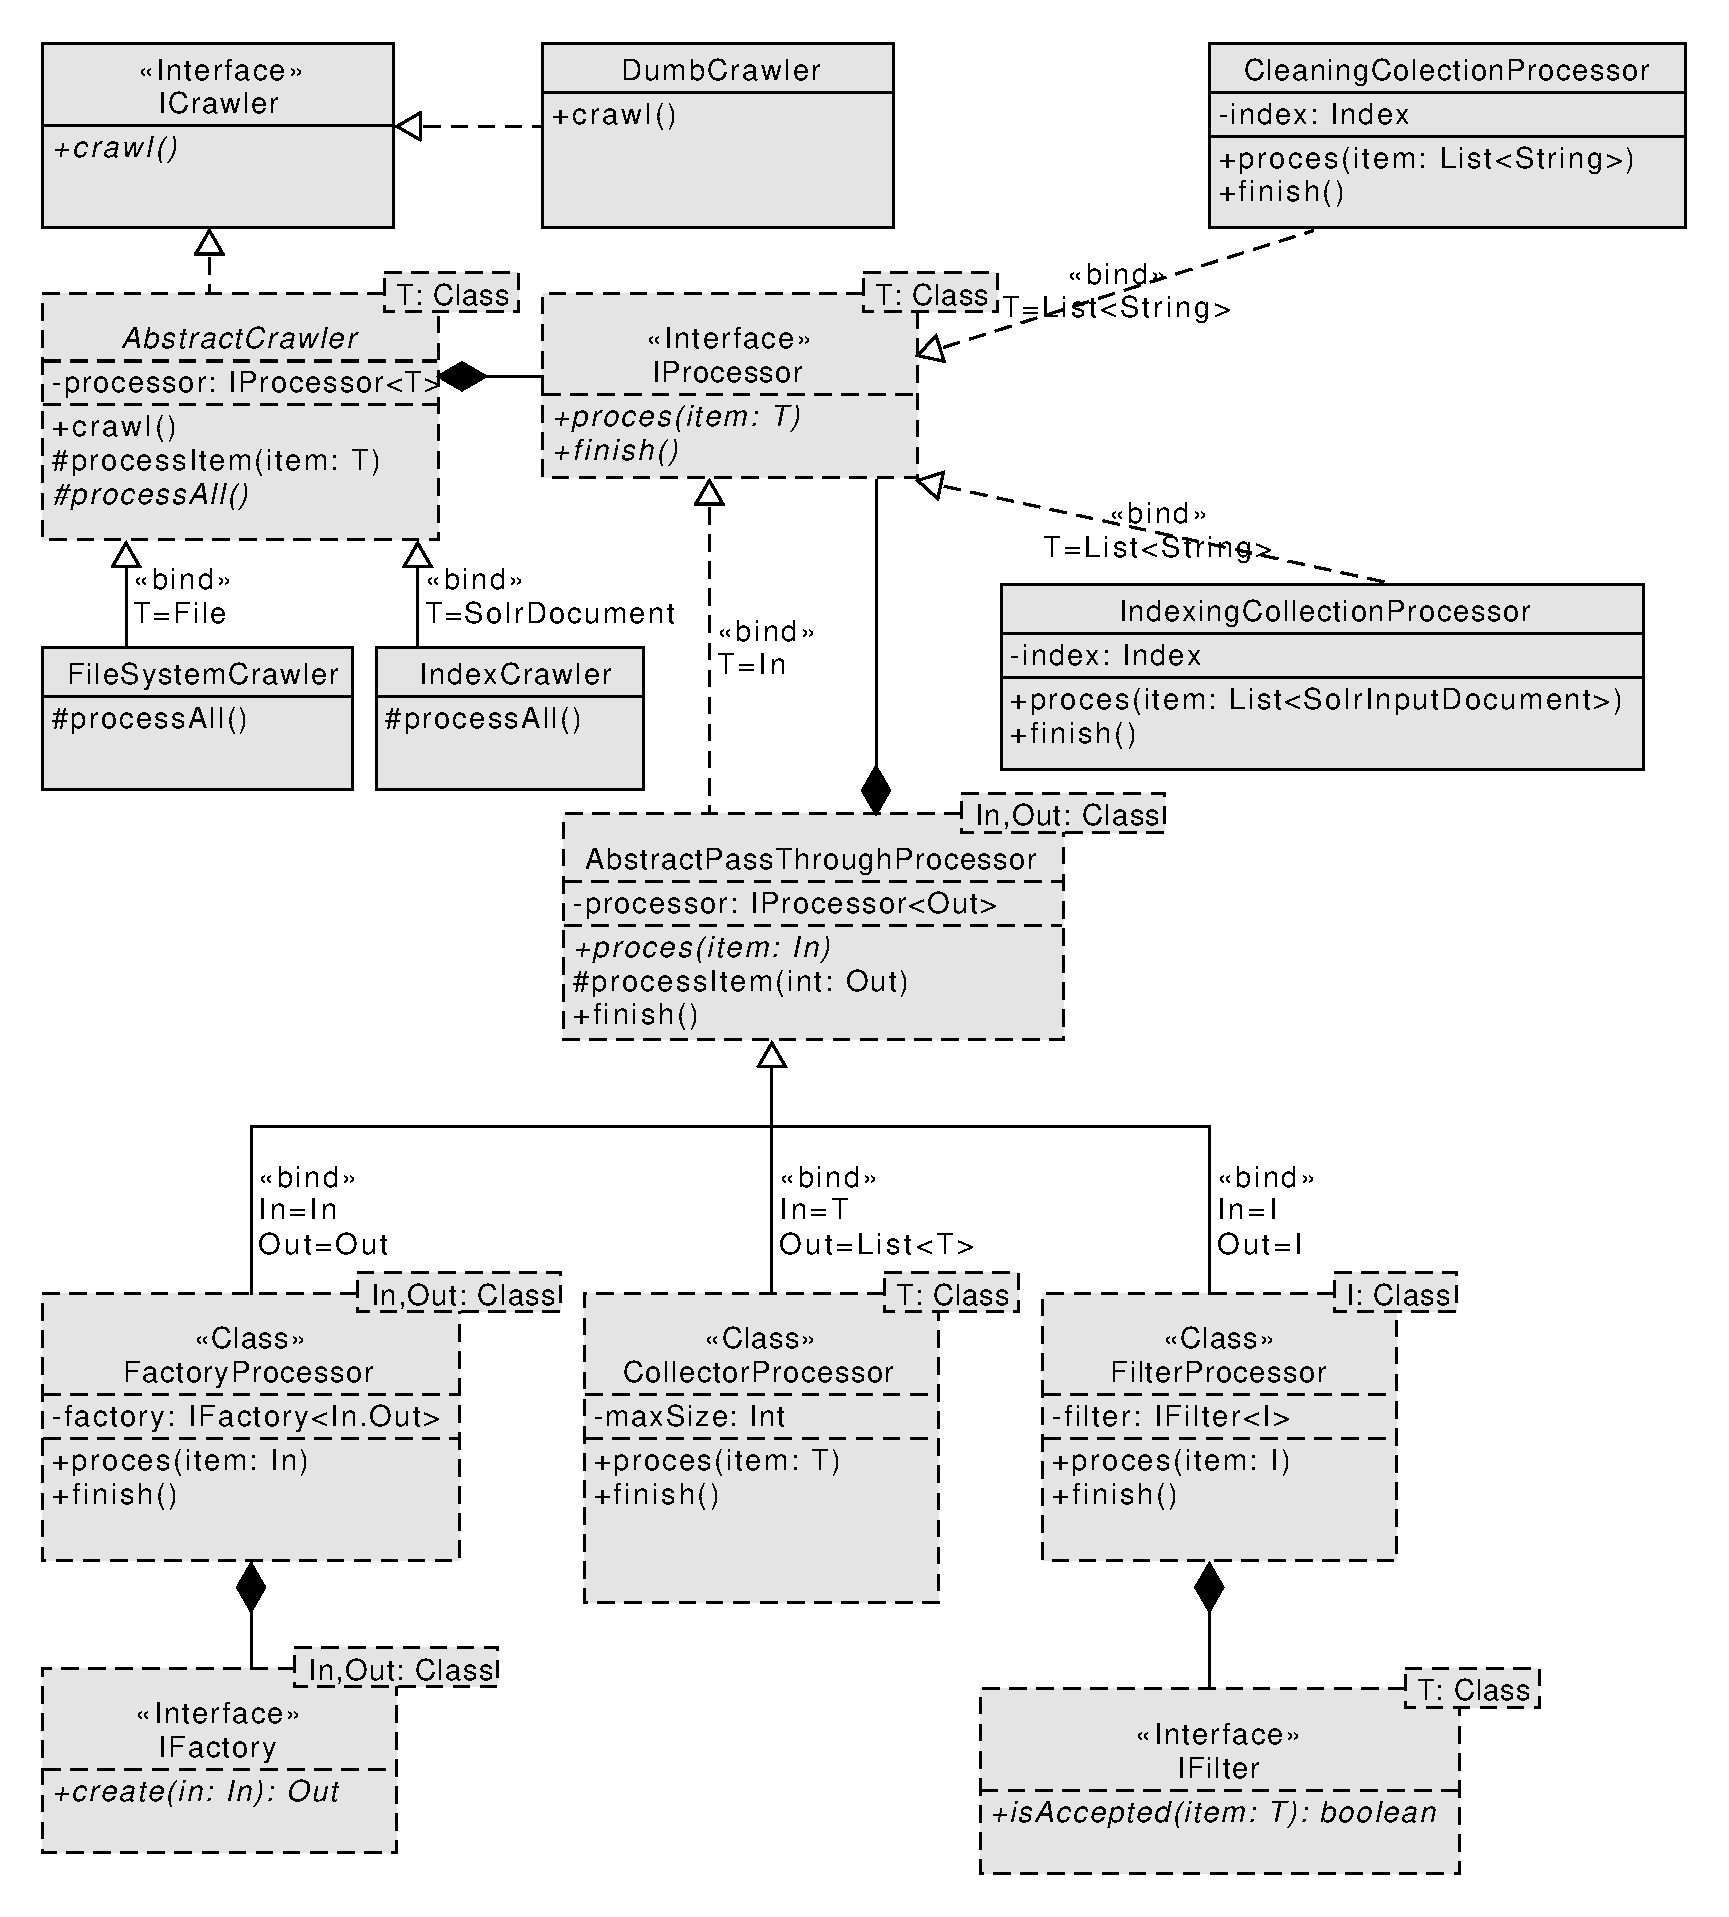
\includegraphics[width=13cm]{ProcessorClasses}
\caption{Diagram procesorových tříd Crawleru}
\label{fig:ProcessorClasses}
\end{center}
\end{figure}

\begin{figure}[h]
\begin{center}
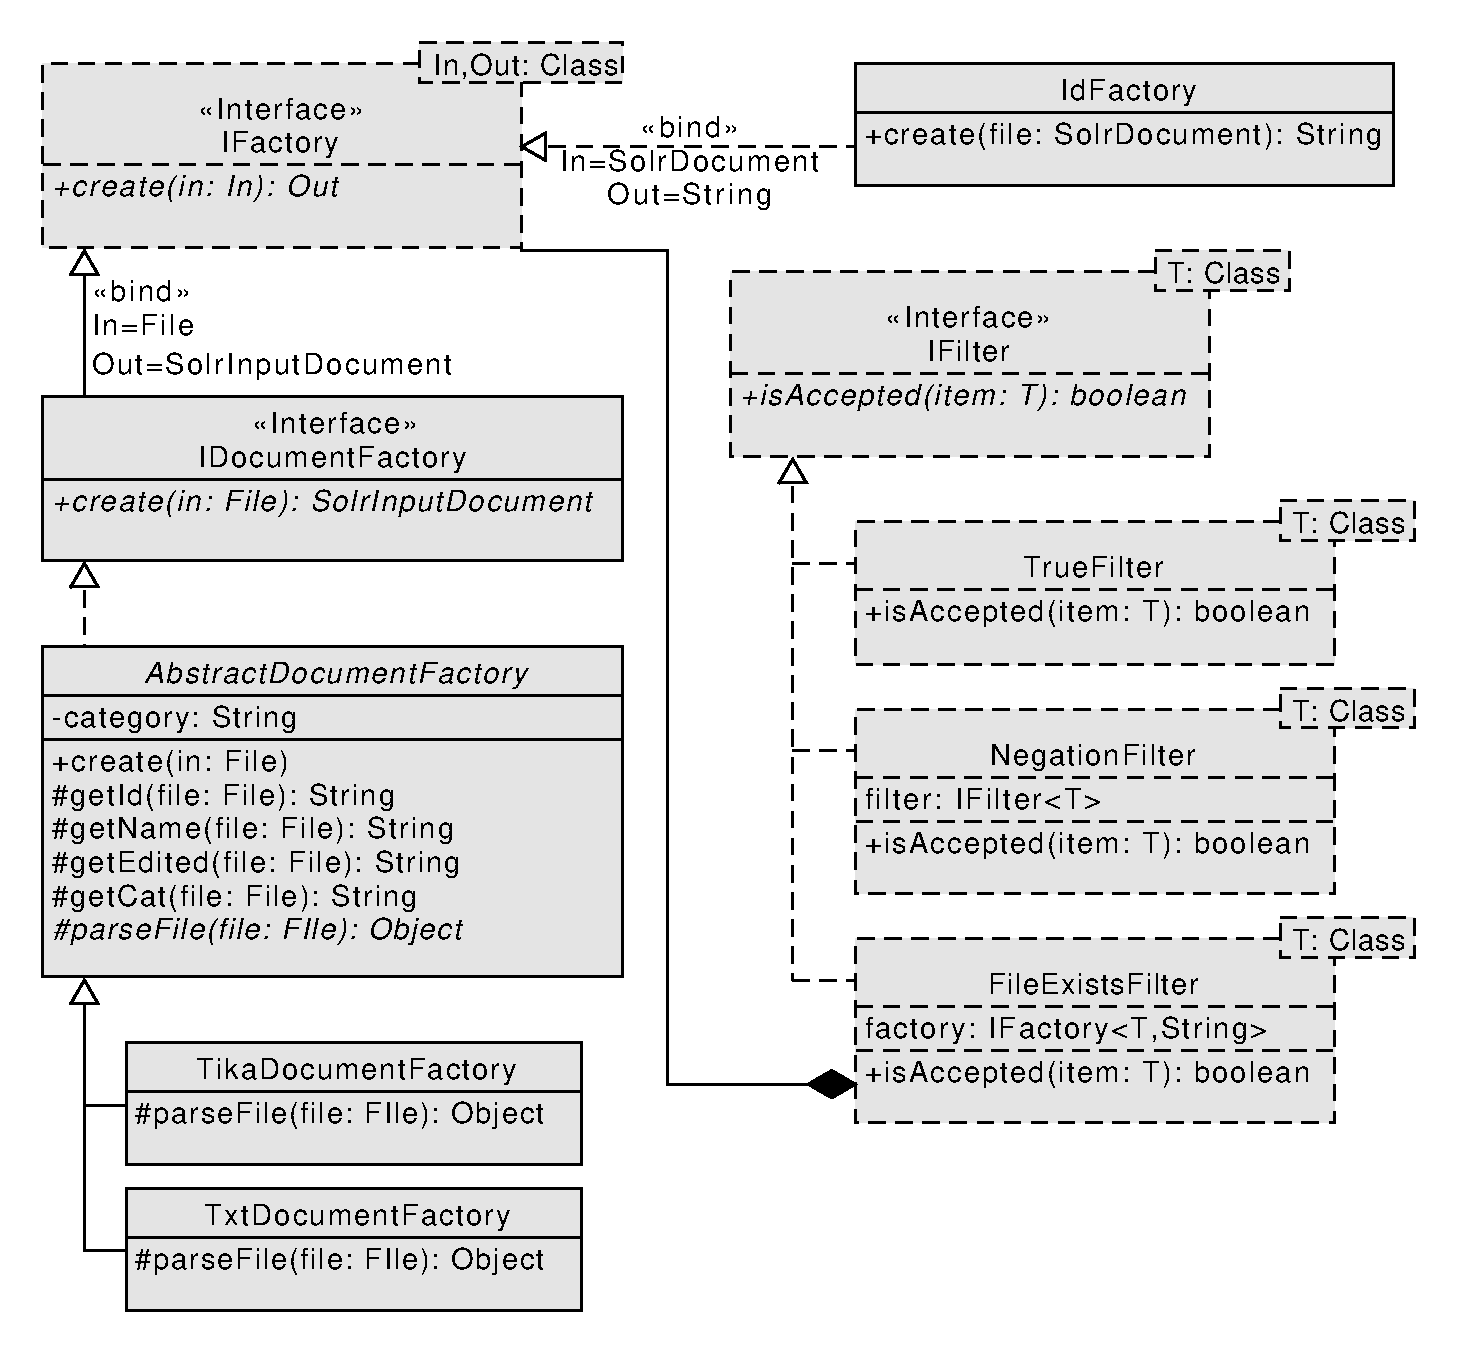
\includegraphics[width=13cm]{OtherClasses}
\caption{Diagram factory a~filter tříd Crawleru}
\label{fig:OtherClasses}
\end{center}
\end{figure}

\subsubsection{Tovární třídy}
Řetězce procesorů budou sestavovány na základě konfigurace, s~využitím návrhového vzoru factory. Sestavování bude mít vždy na starosti daná tovární třída. Tovární třídy se budou řídit parametry přijatými z~konfigurace.

V budoucnosti by bylo možné tyto tovární třídy upravit, aby spolupracovaly s~načítáním tříd a~konfigurací. V~konfiguraci by byl definován řetězec tříd s~případnými konfiguračními parametry. Tovární třída by našla definované třídy (například i~v externích jar knihovnách v~adresáři \emph{lib}), načetla je a~sestavila do řetězce. Tím by byla zaručena absolutní rozšiřitelnost řešení. Podobným způsobem funguje i~konfigurace Solru. Tato verze Crawleru však toto rozšíření zatím obsahovat nebude.

\section{Uživatelské rozhraní} \label{design_frontend}
Na návrhu UI jsem úzce spolupracoval se zadavatelem, abych co nejvíce vyhověl jeho požadavkům. Při návrhu rozhraní jsem se snažil držet se zvyklostí zažitých ve webovém prostředí. Zvláště pak vycházím ze zvyklostí z~internetových vyhledávačů, jako je Google. Další inspirací byl webový frontend aplikace Carrot2. Jelikož jde o~webovou aplikaci, počítá návrh s~proměnnou velikostí okna a~celý layout bude plně responzivní a~přizpůsobitelný pro jakoukoliv velikost okna, včetně mobilní.

Všechny funkční požadavky jde rozdělit do dvou částí: na požadavky týkající se výsledků vyhledávání jako celku (vyhledávání, shlukování) a~požadavky týkající se jednoho vybraného dokumentu (podobnostní vyhledávání, zobrazení obsahu). Uživatelské rozhraní tedy bude sestávat také ze dvou layoutů, z nichž každý bude odpovídat jedné skupině požadavků. Mezi layouty se pak bude volně procházet proklikem. 

Layouty budou mít společný jednotící prvek, a~to hlavičku stránky s~logem aplikace, které bude umístěné tradičně v~levém horním rohu stránky. Zbytek hlavičky bude odpovídat kontextu daného layoutu, aby se neplýtvalo místem. Hlavička bude i~nositelem informace o~kontextu aktuální stránky a~bude napovídat, v~jaké části se uživatel nachází.

\subsection{Vyhledávání dokumentů}
Výchozí stránka bude mít v~hlavičce vyhledávací formulář. Layout je znázorněn na obrázku \ref{fig:SearchLayout}. Formulář bude obsahovat vstupní pole pro výběr zdroje v~podobě roletky, kde uživatel zvolí, který index dokumentů se má pro vyhledávání použít. V~roletce by měl být automaticky vybrán výchozí index nastavený v~Solru. Vpravo od roletky umístím samotné vyhledávací pole a~potvrzovací tlačítko pro vyvolání akce vyhledávání. Vyhledávací pole by mělo být rozměrné a~mělo by vyplnit celou zbývající šířku okna.

\begin{figure}[h]
\begin{center}
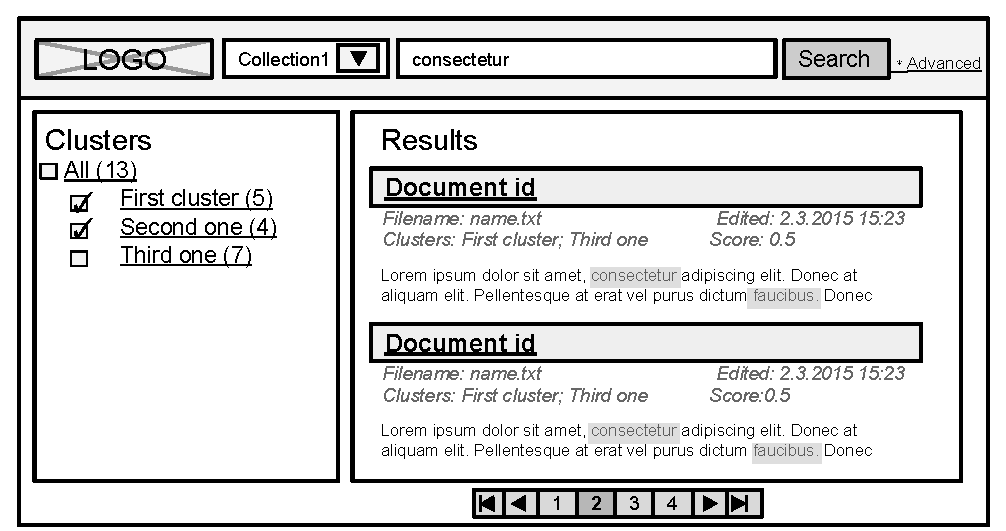
\includegraphics[width=13cm]{SearchLayout}
\caption{Návrh vyhledávacího uživatelského rozhraní}
\label{fig:SearchLayout}
\end{center}
\end{figure}

Vpravo od potvrzovacího tlačítka bude dále umístěn malý odkaz se šipkou, který bude přepínat zobrazení rozšířené nabídky nastavení vyhledávání. Podobu rozšířené nabídky můžeme pozorovat na obrázku \ref{fig:AdvancedLayout}. Nabídka bude stále ještě součástí hlavičky stránky (hlavička se o~ní vlastně rozšíří). Měla by obsahovat jen roletku pro přepínání shlukovacího algoritmu, v~budoucnu bude možné přidat další volby.

\begin{figure}[h]
\begin{center}
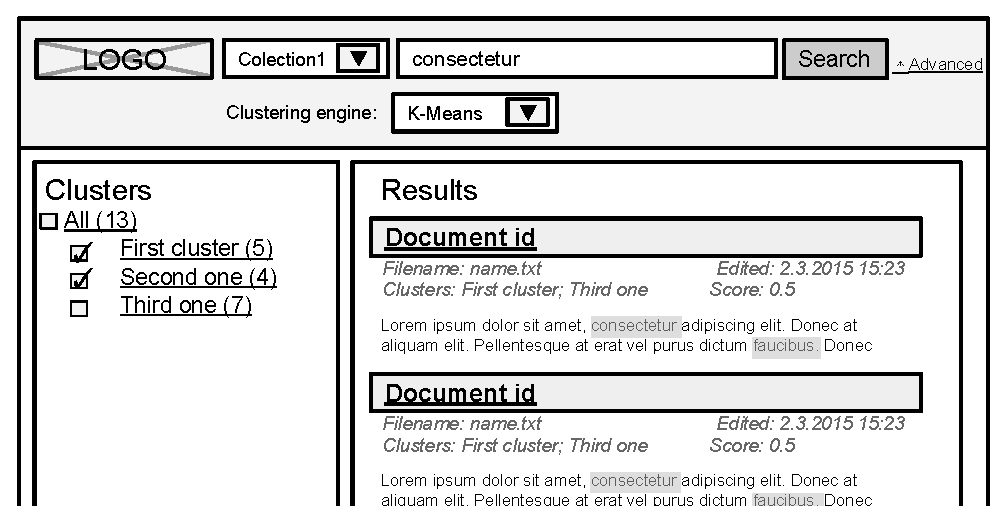
\includegraphics[width=13cm]{AdvancedLayout}
\caption{Návrh vyhledávacího uživatelského rozhraní s~rozšířenou nabídkou}
\label{fig:AdvancedLayout}
\end{center}
\end{figure}

Pod hlavičkou se zobrazí samotný vyhledaný obsah. Všechen vyhledaný obsah projde rovnou shlukovací analýzou. Shlukování nebude nutné zapínat. Vlevo bude umístěn sloupec o~šířce rovné čtvrtině šířky okna s~nalezenými shluky. Vpravo se pak ve zbývající šířce zobrazí nalezené výsledky. Pokud bude okno příliš úzké, zobrazí se výsledky až pod seznamem shluků a~shluky i~výsledky se roztáhnou na plnou šíři okna.

Sloupec se shluky bude mít formu odrážkového seznamu. Nejvyšší prvek seznamu je shluk \uv{All}, který bude obsahovat všechny nalezené výsledky. Pod ním teprve budou jednotlivé nalezené shluky. U~každého shluku se zobrazí číslo odpovídající počtu obsažených dokumentů. Seznam shluků bude provádět i~filtrování dokumentů. Kliknutím na shluk se shluk označí (v obrázku \ref{fig:SearchLayout} je označen zatržítkem) a~ve výsledcích se zobrazí jen dokumenty patřící do vybraného shluku. Vybrat takto půjde libovolný počet shluků. Při každém novém hledání se vždy jako výchozí označí shluk \uv{All}, aby se zobrazily ve výsledcích všechny nalezené dokumenty a~teprve sám uživatel si provedl případnou filtraci.

Sloupec s~výsledky bude obsahovat nalezené dokumenty ve vybraných shlucích. Každý dokument bude reprezentován svým ID v~podobě odkazu vedoucího na zobrazení obsahu dokumentu. Pod ID budou zobrazena různá metadata, jako jméno souboru, kdy byl dokument naposledy upraven, skóre (tj. číslo vyjadřující míru shody hledaného výsledku s~hledaným výrazem) či seznam clusterů, do kterých dokument patří. Pod metadaty bude umístěn úryvek obsahu dokumentu se zvýrazněnými hledanými výrazy. Výsledky budou řazeny podle skóre.

Na konci stránky pod výsledky bude umístěno ovládání stránkování: tlačítka pro posun na předchozí či další stránku, na první či poslední stránku a~seznam několika stránek v~okolí aktuálně zobrazené stránky, která bude na tomto panelu zvýrazněna.

Pořadí sloupců se shluky a~s~výsledky jsem volil s~ohledem na posloupnost pracovního postupu a~na zvyklosti. Lze předpokládat, že uživatel po zadání dotazu nejdříve prohlédne shluky a~vybere, z~kterých shluků chce dokumenty vidět. Seznam shluků má zároveň funkčně nejblíže k~menu, a~to je zvykem na internetových stránkách umisťovat po levé straně od obsahu.

\subsection{Detail dokumentu}
Kliknutím na ID dokumentu ve výsledcích vyhledávání se dostaneme do zobrazení detailu dokumentu. Návrh stránky je znázorněn na obrázku \ref{fig:DetailLayout}. Layout této stránky bude mít v~hlavičce kromě loga už jen vypsané ID otevřeného dokumentu a~bude opět dvousloupcový. Vlevo bude umístěn obsah samotného dokumentu, vpravo sloupec o~šířce jedné třetiny šířky okna obsahující seznam podobných dokumentů k~aktuálně zobrazenému. Bude-li okno příliš malé, sloupce se zobrazí pod sebou na plné šíři okna, stejně jako u~vyhledávacího layoutu. Pořadí sloupců je opět dáno zvyklostmi na internetových stránkách. Sloupec s~podobnými dokumenty se obvykle spolu s~dalšími kontextovými informacemi umisťuje  do pravého sloupce vedle hlavního obsahu, případně pod obsah.

Sloupec s~obsahem bude ve vrchní části zobrazovat metadata dokumentu a~následovat bude celý text dokumentu. Vyhledávané fráze budou v~textu zvýrazněny.

Pravý sloupec bude obsahovat seznam dokumentů, které jsou podobné dokumentu právě otevřenému. Seznam bude strukturován podobně jako seznam výsledků ve vyhledávacím layoutu: bude obsahovat ID dokumentu, které bude zároveň odkazem na detail příslušného dokumentu, poté budou následovat metadata dokumentu a~úryvek obsahu. Dokumenty budou v~tomto sloupci řazeny podle skóre, které vyjadřuje míru podobnosti dokumentu s~otevřeným dokumentem.

\begin{figure}[h]
\begin{center}
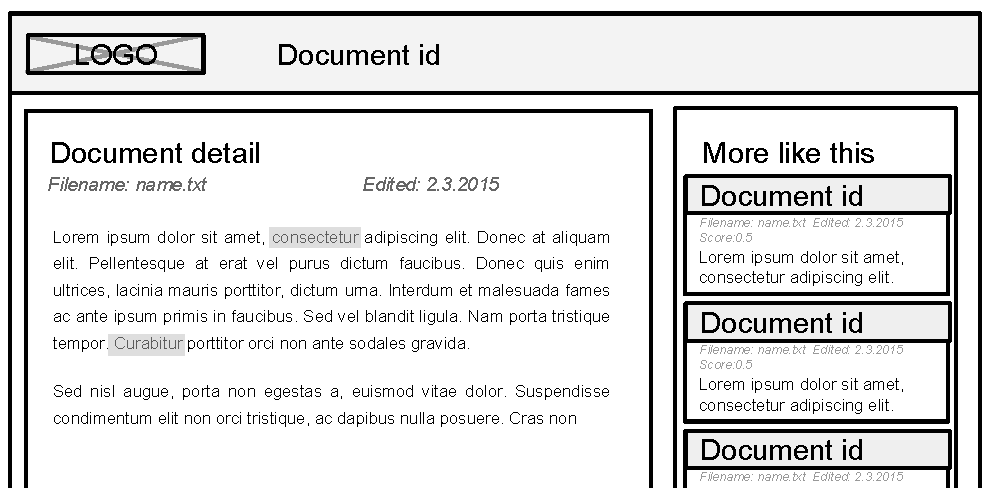
\includegraphics[width=13cm]{DetailLayout}
\caption{Návrh uživatelského rozhraní pro zobrazení dokumentu}
\label{fig:DetailLayout}
\end{center}
\end{figure}
\chapter{Implementace}
\section{Solr}
Základní komponentou, kterou bylo třeba implementovat, byl Solr. Potřebuji aby software zvládl indexovat text v~českém jazyce. Solr obsahuje předinstalovanou a~částečně předkonfigurovanou českou sadou analyzerů, která zahrnuje \emph{StandardTokenizer}, \emph{LowerCaseFilter}, \emph{StopFilter} a \emph{CzechStemFilter}. V~tomto pořadí.

\emph{StandardTokenizer} dělí text na tokeny. Po zběžné zkoušce jsem usoudil, že heho algoritmus je funkční i~pro český jazyk. \emph{LowerCaseFilter} je určen k převodu textu na malá písmena. I tento filtr jsem také otestoval a~opět se neprojevily žádné problémy --- převádí na malá písmena i~speciální české znaky s~interpunkcí. 

\emph{StopFilter} odebírá tokeny odpovídající seznamu. Jeho fungování tedy závisí na kvalitě seznamu. V~Solru je předinstalován seznam \emph{czech\_stopwords.txt}, jenž obsahuje slova, která jsou v českém jazyce natolik frekventovaná, že nevypoví o vyhledávaném textu žádnou zásadní informaci. Jedná se především o nejrůznější předložky, spojky a~pomocná slovesa. Tento seznam jsem shledal dostačujícím, už proto, že kdykoliv v~případě potřeby půjde seznam rozšířit o~další slova, která se vyskytují příliš často v~policejním prostředí, a~nepomáhají tudíž specifikovat hledaný text.

Poslední \emph{CzechStemFilter} je klíčový analyzer. Jak jsem již psal v~kapitole \ref{analysis}~Analýza, měl by být výsledkem práce švýcarských programátorů. O jeho kvalitách nejsem zcela přesvědčen, implementoval jsem proto do Solru další české stemmery.

\subsection{Stemmery}
K~tomu, aby mohl být implementovaný \emph{StemFilter} použit v~Solru, je nutno vytvořit JAR knihovnu obsahující třídu implementující rozhraní \emph{TokenFilter} a~zároveň její tovární třídu, nejlépe potomka \emph{TokenFilterFactory}. Sestavená JAR knihovna se pak umístí do adresáře \emph{Lib}, kde z~ní bude moci \emph{ClassLoader} Solru číst. V~konfiguraci Solru je pak již možné použít nový filtr definovaný absolutním jménem tovární třídy. Parametry definované v~konfiguraci se předávají tovární třídě, je tedy možné konfigurací ovlivnit funkci stemmeru.

\subsubsection{Light a~Agressive stemmer}
Vnitřní \emph{CzechStemFilter} Solru je dle dokumentace\cite{sorl:doc} jedním ze stemizačních algoritmů autorů L.~Dolamica a~J.~Savoye. Výsledkem jejich práce \cite{Dolamic:2009:Stemming} je stemizační algoritmus, který je založen na technice postupného hledání a~odtrhávání koncovek slov. Vytvořili dvě verze svého algoritmu, takzvanou light a~agressive verzi, které se liší počtem odebíraných koncovek slov (agresivní verze jich odebírá více). Ani jedna z~těchto verzí ale prostým porovnáním kódu neodpovídá českému filtru implementovanému v~Solru. Rozhodl jsem se proto, že doimplementuji light i~agressive stemmer.

Zdrojový kód obou stemmerů je k~dispozici na internetu v~jazyce Java pod BSD licencí. Jde o~dvě třídy s~implementací. Vytvořil jsem tedy vlastní třídu \emph{CzechStemFilter}, která bude tvořit adaptér implementačním třídám. Dále jsem vytvořil tovární třídu \emph{CzechStemFilterFactory}, která inicializuje \emph{CzechStemFilter} a~dle parametrů v~konfiguraci zvolí „agresivní“ či „odlehčenou“ implementaci stemmeru. Při tvorbě těchto dvou tříd jsem se inspiroval původní implementací \emph{CzechStemFilter} v~aplikaci Solr.

Výslednou implementaci jsem zkompiloval do knihovny \emph{Analyzery.jar} a~podle výše popsaného postupu integroval do Solru.

\subsubsection{Helebrand stemmer}
V rámci dalšího výzkumu jsem nalezl diplomovou práci D.~Helebranda z~VUT v~Brně\cite{Helebrand:2010:Stemming}, který implementoval stemmer pro český jazyk v~prostředí Snowball. Snowball je programovací jazyk speciálně navržený pro zpracovávání textových řetězců, především právě pro tvorbu stemizačních algoritmů. Výsledný algoritmus lze pomocí nástrojů Snowballu přímo přeložit do jazyka C či Java. Hotový stemizační algoritmus pana Helebranda je k~dispozici pod licencí GNU General Public License.

Získal jsem tedy algoritmus z~webových stránek brněnské technické univerzity a~pomocí výše zmíněných nástrojů jsem jej nechal přeložit do Javy. Solr v~sobě již má implementovány stemmery pro několik jazyků pomocí prostředí Snowball, nebylo proto příliš složité výsledný Java algoritmus integrovat. Obsažená tovární třída \emph{SnowballPorterFilterFactory} je příhodně navržená tak, že jméno  portované třídy s~algoritmem hledá v~balíčku \emph{org.tartarus.snowball.ext}. Stačilo tedy jen vygenerovanou třídu s~algoritmem vhodně pojmenovat a~umístit do správného balíčku. \emph{SnowballPorterFilterFactory} přijímá jméno třídy, kterou má hledat, jako parametr z~konfigurace.

Výslednou sestavu jsem přibalil do JAR knihovny s~předchozími implementacemi stemmerů, bude tedy umístěna v~adresáři \emph{Lib}, kde ji \emph{ClassLoader} Solru nalezne.

\subsubsection{Hunspell stemmer}
Po implementaci tří stemmerů založených na postupném odtrhávání koncovek jsem začal hledat řešení, které by používalo jinou metodu získávání kořenů. Hledal jsem algoritmus založený buď na strojovém učení, nebo na porovnávání se slovníkem a zjistil jsem, že existuje algoritmus, který využívá Hunspell k~odebrání koncovek s~využitím slovníku, a~že je již implementovaný v~Solru.

Hunspell je opensource knihovna sloužící ke kontrole pravopisu. Je využívaný například v~projektech Apache OpenOffice či Google Chrome. Slovníky, včetně českého, lze pro Hunspell volně stáhnout přímo z~internetových stránek OpenOffice\cite{openoffice}. České slovníky jsou licencovány pod GNU/GPL licencí. Byly tvořeny pro starší knihovnu Ispell, Hunspell je s ní však zpětně kompatibilní.

Ze sady souborů českého slovníku v projektu využiji jen dva: soubor s~koncovkou \emph{.dic}, který obsahuje seznam slov daného jazyka, ideálně v~kořenovém tvaru, a~soubor \emph{.aff}, který obsahuje pravila přidávání koncovek\cite{zdrojak}. Soubor \emph{cs\_CZ.aff} českého slovníku obsahuje syntaktickou chybu, kterou jsem musel před použitím slovníku opravit, protože jinak se Solr při jeho „parsování“ ukončí kritickou chybou.

Nevýhodu této metody vidím především v~nedostatečné kvalitě slovníku. Poslední verze pochází z~roku 2008 a~nezdá se, že by byl nadále aktivně rozšiřován.

\subsection{Konfigurace} \label{sorlconfig}
\subsubsection{Datová pole}
K již existujícímu textovímu datovému typu \emph{text\_cz}, který používá vestavěný český stemmer, jsem v konfiguračním souboru \emph{schema.xml} vytvořil datové typy, jenž využívají nově vytvořené stemmery. Toho jsem docílil následující konfigurací.

\begin{verbatim}
<!-- Czech original -->
<fieldType name="text_cz" 
           class="solr.TextField" 
           positionIncrementGap="100">
  <analyzer> 
    <tokenizer class="solr.StandardTokenizerFactory"/>
    <filter class="solr.LowerCaseFilterFactory"/>
    <filter class="solr.StopFilterFactory" 
            ignoreCase="true" 
            words="lang/stopwords_cz.txt" />
    <filter class="solr.CzechStemFilterFactory"/>       
  </analyzer>
</fieldType>

<!-- Czech Helebrand -->
<fieldType name="text_cz_helebrand" 
           class="solr.TextField" 
           positionIncrementGap="100">
  <analyzer> 
    <tokenizer class="solr.StandardTokenizerFactory"/>
    <filter class="solr.LowerCaseFilterFactory"/>
    <filter class="solr.StopFilterFactory" 
            ignoreCase="true" 
            words="lang/stopwords_cz.txt" />
    <filter class="solr.SnowballPorterFilterFactory" 
            language="CzechHelebrand" />       
  </analyzer>
</fieldType>

<!-- Czech Dolamic light-->
<fieldType name="text_cz_light" 
           class="solr.TextField"
           positionIncrementGap="100">
  <analyzer> 
    <tokenizer class="solr.StandardTokenizerFactory"/>
    <filter class="solr.LowerCaseFilterFactory"/>
    <filter class="solr.StopFilterFactory" 
            ignoreCase="true" 
            words="lang/stopwords_cz.txt" />
    <filter class=
"cz.cvut.skorpste.dip.stemmer.dolamicsavoy.CzechStemFilterFactory" 
            implementation="Light" />       
  </analyzer>
</fieldType>

<!-- Czech Dolamic agressive-->
<fieldType name="text_cz_agressive" 
           class="solr.TextField" 
           positionIncrementGap="100">
  <analyzer> 
    <tokenizer class="solr.StandardTokenizerFactory"/>
    <filter class="solr.LowerCaseFilterFactory"/>
    <filter class="solr.StopFilterFactory"
            ignoreCase="true" 
            words="lang/stopwords_cz.txt" />
    <filter class=
"cz.cvut.skorpste.dip.stemmer.dolamicsavoy.CzechStemFilterFactory"
       	   implementation="Agressive" />       
  </analyzer>
</fieldType>

<!-- Czech Hunspell -->
<fieldType name="text_cz_hunspell" 
           class="solr.TextField" 
           positionIncrementGap="100">
  <analyzer> 
    <tokenizer class="solr.StandardTokenizerFactory"/>
    <filter class="solr.LowerCaseFilterFactory"/>
    <filter class="solr.StopFilterFactory" 
            ignoreCase="true" 
            words="lang/stopwords_cz.txt" />
    <filter class="solr.HunspellStemFilterFactory" 
            dictionary="cs_CZ.dic" affix="cs_CZ.aff" />       
  </analyzer>
</fieldType>
\end{verbatim}

Datové typy jsou pojmenované \emph{text\_cz\_light}, \emph{text\_cz\_agressive}, \emph{text\_cz\_helebrand} a~\emph{text\_cz\_hunspell}. Všechny tyto typy mají shodný analyzer pro dotazování i~pro indexování. V~ukázce konfigurace můžeme pozorovat parametry stemmerů, o~kterých jsem se zmiňoval v~kapitolách o~implementaci jednotlivých stemmerů.

Poté jsem definoval datová pole indexu. Pole se definují také v~konfiguračním souboru \emph{schema.xml}. Pole ID je povinné, protože (podobně jako v~databázích) jednoznačně identifikuje dokument. Datový typ tohoto pole jsem nastavil na \emph{string} a~budu do něj ukládat absolutní cestu k~souboru ve filesystému zdrojového počítače. Pole \emph{name} bude uchovávat jméno souboru, ze kterého dokument pochází, pole \emph{edited} pak čas poslední editce souboru. Pole \emph{cat} je spíše přípravou pro budoucí možnost rozšíření o nastavení kategorie, do které soubor spadá. Aktuálně nemá žádnou funkci.

Posledním definovaným polem je \emph{text}, do kterého se bude ukládat samotný text dokumentu. Jeho datový typ je aktuálně nastavený na \emph{text\_cz} a~lze jej nastavit na kterýkoliv z~implementovaných českých datových typů definovaných výše. O tom, který datový typ bude zvolen ve výchozím nastavení, rozhodnu na základě výsledků testu stemmerů v~kapitole \ref{testing} Testování. 

\begin{verbatim}
<field name="id" type="string" indexed="true" 
       stored="true" required="true" 
       multiValued="false" /> 
<field name="name" type="text_general" indexed="true" 
       stored="true"/>
<field name="edited" type="date" indexed="true" 
       stored="true" />
<field name="cat" type="string" indexed="true" 
       stored="true" required="true" multiValued="false"/>
<field name="text" type="text_cz" indexed="true" 
       stored="true" termVectors="true" />
\end{verbatim}

\subsubsection{Request handlery}
Konfigurace tzv. request handlerů se nalézá v~konfiguračním souboru \emph{solrconfig.xml}. Mapuje URL adresu na komponenty, které dle nastavení zpracují požadavek. Definoval jsem dva request handlery, z nichž každý odpovídá jedné stránce uživatelského rozhraní, protože pro každou stránku bude třeba jiné zpracování. 

Request handler \emph{/searcher} je určen pro stránku vyhledávání a~bude tedy dodávat výsledky vyhledávání obohacené o~shlukování a zvýraznění hledaných slov. Dále se v~konfiguraci nastavuje výchozí velikost stránky, výchozí dotaz a pole, která má server vrátit v odpovědi. Druhý request handler, \emph{/detail}, je určen pro stránku s~detailem o~dokumentu a~bude tedy vracet obsah dokumentu se zvýrazněním hledaných slov a~podobné dokumenty.

\begin{verbatim}
<requestHandler name="/searcher"
                startup="lazy"
                enable="${solr.clustering.enabled:false}"
                class="solr.SearchHandler">
  <lst name="defaults">
  
    <!-- Clustering -->
    <bool name="clustering">true</bool>
    <bool name="clustering.results">true</bool>
    <bool name="clustering.collection">true</bool>
    <str  name="clustering.engine">lingo</str>
    <str name="carrot.title">text</str>
    <str name="carrot.url">id</str>
    <bool name="carrot.produceSummary">true</bool>
    <bool name="carrot.outputSubClusters">true</bool>
    
    <!-- Search -->
    <str name="defType">edismax</str>
    <str name="qf">text^10.0</str>
    <str name="df">text</str>
    <str name="mm">100%</str>
    <str name="q.alt">*:*</str>
    <str name="rows">50</str>
    <str name="fl">*,score</str>
    
    <!-- More like this -->
    <str name="mlt.qf">text^10.0</str>
    <str name="mlt.fl">text</str>
    <int name="mlt.count">0</int>
    
    <!-- Highlighting -->
    <str name="hl">on</str>
    <str name="hl.fl">text</str>
    <str name="hl.preserveMulti">true</str>
    <str name="hl.encoder">html</str>
    <str name="hl.simple.pre">&lt;mark&gt;</str>
    <str name="hl.simple.post">&lt;/mark&gt;</str>
    <str name="hl.simple.ellipsis">…</str>
    <str name="f.text.hl.snippets">3</str>
    <str name="f.text.hl.fragsize">200</str>
    <str name="f.text.hl.alternateField">text</str>
    <str name="f.text.hl.maxAlternateFieldLength">750</str>
  </lst>
  <arr name="last-components">
    <str>clustering</str>
  </arr>
</requestHandler>

<requestHandler name="/detail"
                startup="lazy"
                class="solr.SearchHandler">
  <lst name="defaults">
  
    <!-- Search -->
    <str name="defType">edismax</str>
    <str name="qf">text^10.0</str>
    <str name="df">text</str>
    <str name="mm">100%</str>
    <str name="q.alt">*:*</str>
    <str name="rows">1</str>
    <str name="fl">*,score</str>
    
    
    <!-- More like this -->
    <str name="mlt">true</str>
    <str name="mlt.qf">text^10.0</str>
    <str name="mlt.fl">text</str>
    <int name="mlt.count">10</int>
    
    <!-- Highlighting -->
    <str name="hl">on</str>
    <str name="hl.fl">text</str>
    <str name="hl.preserveMulti">true</str>
    <str name="hl.encoder">html</str>
    <str name="hl.simple.pre">&lt;mark&gt;</str>
    <str name="hl.simple.post">&lt;/mark&gt;</str>
    <str name="hl.simple.ellipsis">…</str>
    <str name="f.text.hl.snippets">1</str>
    <str name="f.text.hl.fragsize">0</str>
    <str name="f.text.hl.alternateField">text</str>
    <str name="f.text.hl.maxAlternateFieldLength">0</str>
  </lst>
</requestHandler>
\end{verbatim}

\section{Crawler}
Crawler jsem implementoval přesně podle návrhu popsaného v kapitole \ref{design_crawler}. Třída\emph{DocumentFactory} tvoří výsledné dokumenty odpovídající schématu Solru a~aplikace počítá při ověřování existence souboru s~tím, že v~poli \emph{id} je uložena absolutní cesta k~souboru v~místním filesystému.

\subsection{Konfigurace}
Veškerá konfigurace se realizuje pomocí Apache commons-config knihovny. Knihovna umožňuje načíst a zparsovat hned několik zdrojů nastavení a pak v místě potřeby jen získat hodnotu pomocí definovaného klíče. Za sestavení konfigurace je zodpovědná třída \emph{ConfigFactory}. Ta vrací singleton objekt \emph{Config} s nastavením.

Crawler nastavení načítá z parametrů Java VM, z konfiguračního souboru a z vnitřního konfiguračního souboru. Tyto soubory jsou ve formátu Java properties. Hodnoty nastavení lze přetěžovat s tím, že nejvyšší prioritu mají parametry VM, poté soubor a nejnižší prioritu má vnitřní konfigurační soubor. Cestu k souboru s nastavením lze dodat programu pomocí VM parametru. Bez tohoto parametru se aplikace pokusí načíst konfiguraci ze souboru \emph{crawler.properties}. Pokud soubor nenalezne, nastavení ze souboru nenačte vůbec a chování se bude řídit pouze pomocí parametrů předaných Java VM a vnitřním souborem s nastavením.

Kromě adresy Solr serveru a umístění konfiguračního souboru řídí konfigurace také sestavování  řetězců procesorů a obsahuje tedy informace pro tovární třídy, které řetězce sestavují. Řetězce jsou dva, proto jsou nastaveny ve dvou prefixech \verb|indexer| a \verb|cleaner|. V každém prefixu jsou pak uloženy informace pro jednotlivé části řetězce. Příklady sestavených řetězců jsou znázorněny na diagramu\ref{fig:ProcessorChain}. Zobrazené řetězce indexing a cleaning se sestavují ve výchozí konfiguraci, a jejich tvorba je tedy definovaná ve vnitřním souboru \emph{config.properties}.

\begin{figure}[h]
\begin{center}
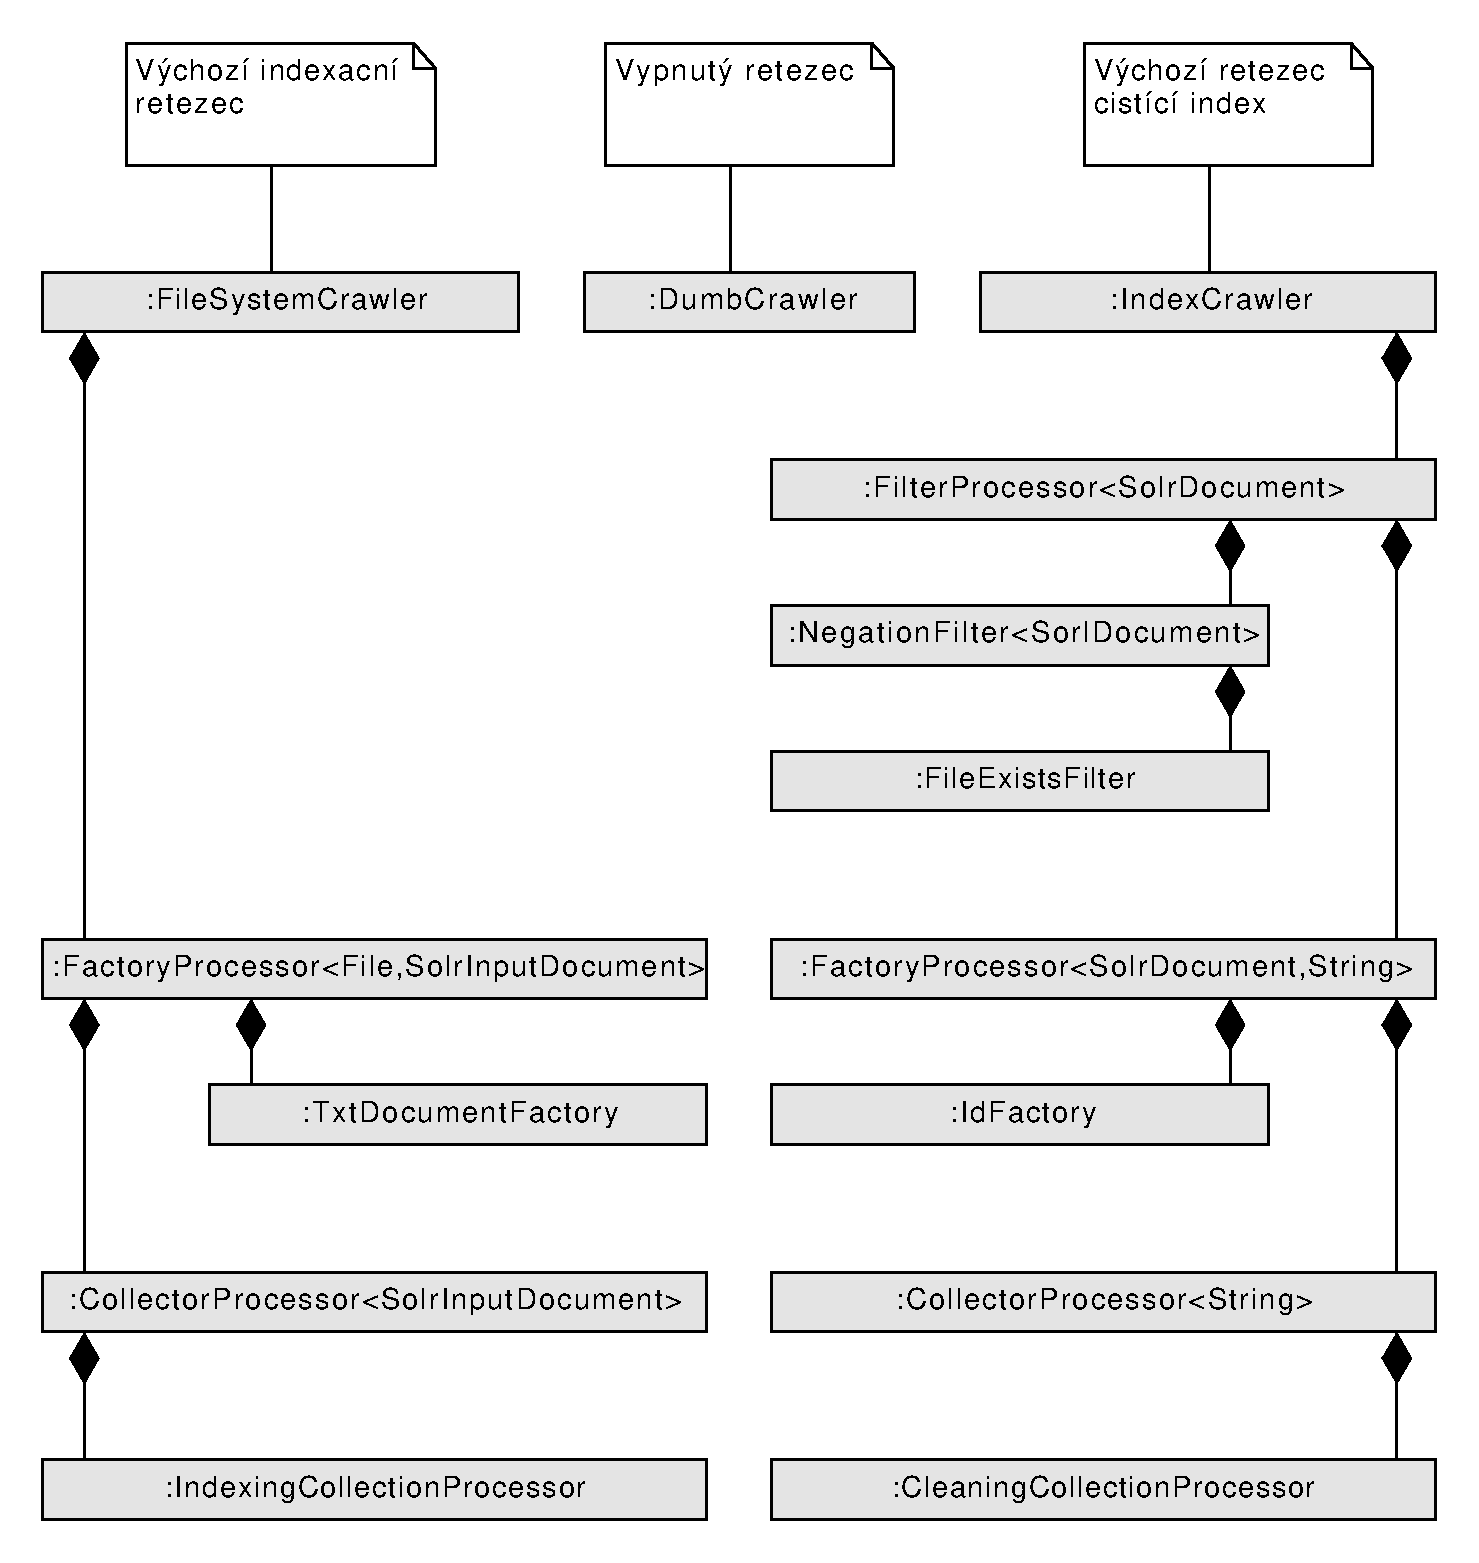
\includegraphics[width=13cm]{ProcessorChain}
\caption{Objektový model sestavených procesorových řetězů Crawleru}
\label{fig:ProcessorChain}
\end{center}
\end{figure}


\subsection{Sestavení}
Kompilace aplikace je nastavena tak, aby se vytvořil JAR soubor obsahující všechny knihovny, na kterých aplikace závisí. K~aplikaci jsem vytvořil skript pro prostředí Windows i~Linux, který zjednoduší její spouštění.

\section{Frontend}
Frontend podle návrhu sestává ze dvou statických HTML stránek oživených pomocí JavaScriptu. Pro usnadnění tvorby layoutu jsem využil CSS knihovny Bootstrap\cite{bootstrap}, která přináší jednotný a~přehledný vizuální styl a~definuje vizuální komponenty nad rámec prostého HTML.

Stránku jsem oživil pomocí JavaScriptové knihovny Angular.js\cite{angular}, která mi umožnila provázat backend v~podobě Solru s~HTML frontendem za použití služeb pro JSON komunikaci se serverem a~tzv. two way bindingu, mechanismu k~provázání HTML DOM s~JavaScriptovým modelem. Angular.js zastoupil i původní JavaScriptovou knihovnu Bootstrapu, protože umožňuje definovat mnohem jednodušším způsobem i skrývání komponent a prvků v návaznosti na události.

Oproti popsanému návrhu v kapitole \ref{design_frontend} jsem opatřil prvky ikonami ze sady volně použitelných univerzálních ikon FontAwesome\cite{fontawesome}, které usnadní vizuální navigaci uživatele po stránce. Ikonami jsem nahradil i původně zamýšlené zaškrtávací vstupní pole u jednotlivých shluků. Použil jsem ikonu adresáře, kterou uživatelé znají a která napoví, že položky znázorňují jisté skupiny dokumentů. Vybrané shluky se znázorní ikonou adresáře otevřeného. Číselné vyjádření počtu dokumentů ve shluku jsem umístil do komponenty \emph{badge}, kterou je zvykem na internetu používat k tomuto účelu. Seznam shluků, do kterých patří dokumenty ve výsledcích, jsou umístěné ve vizuální komponentě \emph{label}, kterou je zvykem používat například pro zobrazení štítků u položek. Výsledný layout lze vidět na obrázcích \ref{fig:ScreenSearcher} a~\ref{fig:ScreenDetail}.

Aplikace počítá s~nasazením aplikace Solr na stejném webovém serveru. Služby načítající data se přímo odkazují na request handlery \emph{/solr/searcher} a~\emph{/solr/detail} definované v kapitole \ref{sorlconfig}, a~kromě toho získávají data o~dostupných indexech pomocí vnitřního handleru \emph{/solr/admin/cores}.

Při implementaci jsem dbal na to, aby web odpovídal běžným zvyklostem i přesto, že je implementovaný v~JavaScriptu. Všechny změny stavu aplikace jsou proto promítány i~do adresního řádku. Díky tomu lze například zkopírováním adresy odkazovat na konkrétní výsledky vyhledávání, využívat funkcí zpět a~vpřed v~historii prohlížeče, či otevírat odkazy v~novém okně pomocí běžných prostředků prohlížeče. Využívám k~tomu standardní \emph{Angular.js} službu \emph{Route}, která zprostředkovává parsování i~změny informací v~adresním řádku.

Aby mohl být frontend nasazen do servlet containeru, umístil jsem všechny statické soubory do adresáře \emph{webapp} webové aplikace a~vytvořil \emph{HttpServlet} pojmenovaný \emph{ViewFile}, jehož jedinou funkcí je odeslat jako odpověď obsah souboru. V~konfiguračním souboru \emph{WEB-INF/web.xml} jsem servlet zaregistroval a~namapoval na něj všechny url adresy. Výsledná aplikace se kompiluje jako WAR soubor, který je možné nasadit do servlet containeru.

\begin{verbatim}
<servlet>
  <servlet-name>ViewFile</servlet-name>
  <servlet-class>cz.cvut.skorpste.dip.frontend.ViewFile</servlet-class>
</servlet>

<servlet-mapping>
  <servlet-name>ViewFile</servlet-name>
  <url-pattern>/*</url-pattern>
</servlet-mapping>
\end{verbatim}

\section{Jetty}
Posledním krokem v rámci implementace řešení byla konfigurace serveru Jetty. Použil jsem instalaci distribuovanou se Solrem. Port serveru jsem nastavil na 8080 místo standardního 80, abych minimalizoval kolizi s~jiným webovým serverem, a~aby pro běh aplikace nebyly zapotřebí práva správce. Do aplikace jsem přidal webovou aplikaci \emph{frontend} a~nastavil \emph{contextPath} na kořenový adresář serveru. Pro usnadnění spouštění aplikace jsem napsal krátké scripty pro prostředí Linux i~Windows.

\begin{figure}[h]
\begin{center}
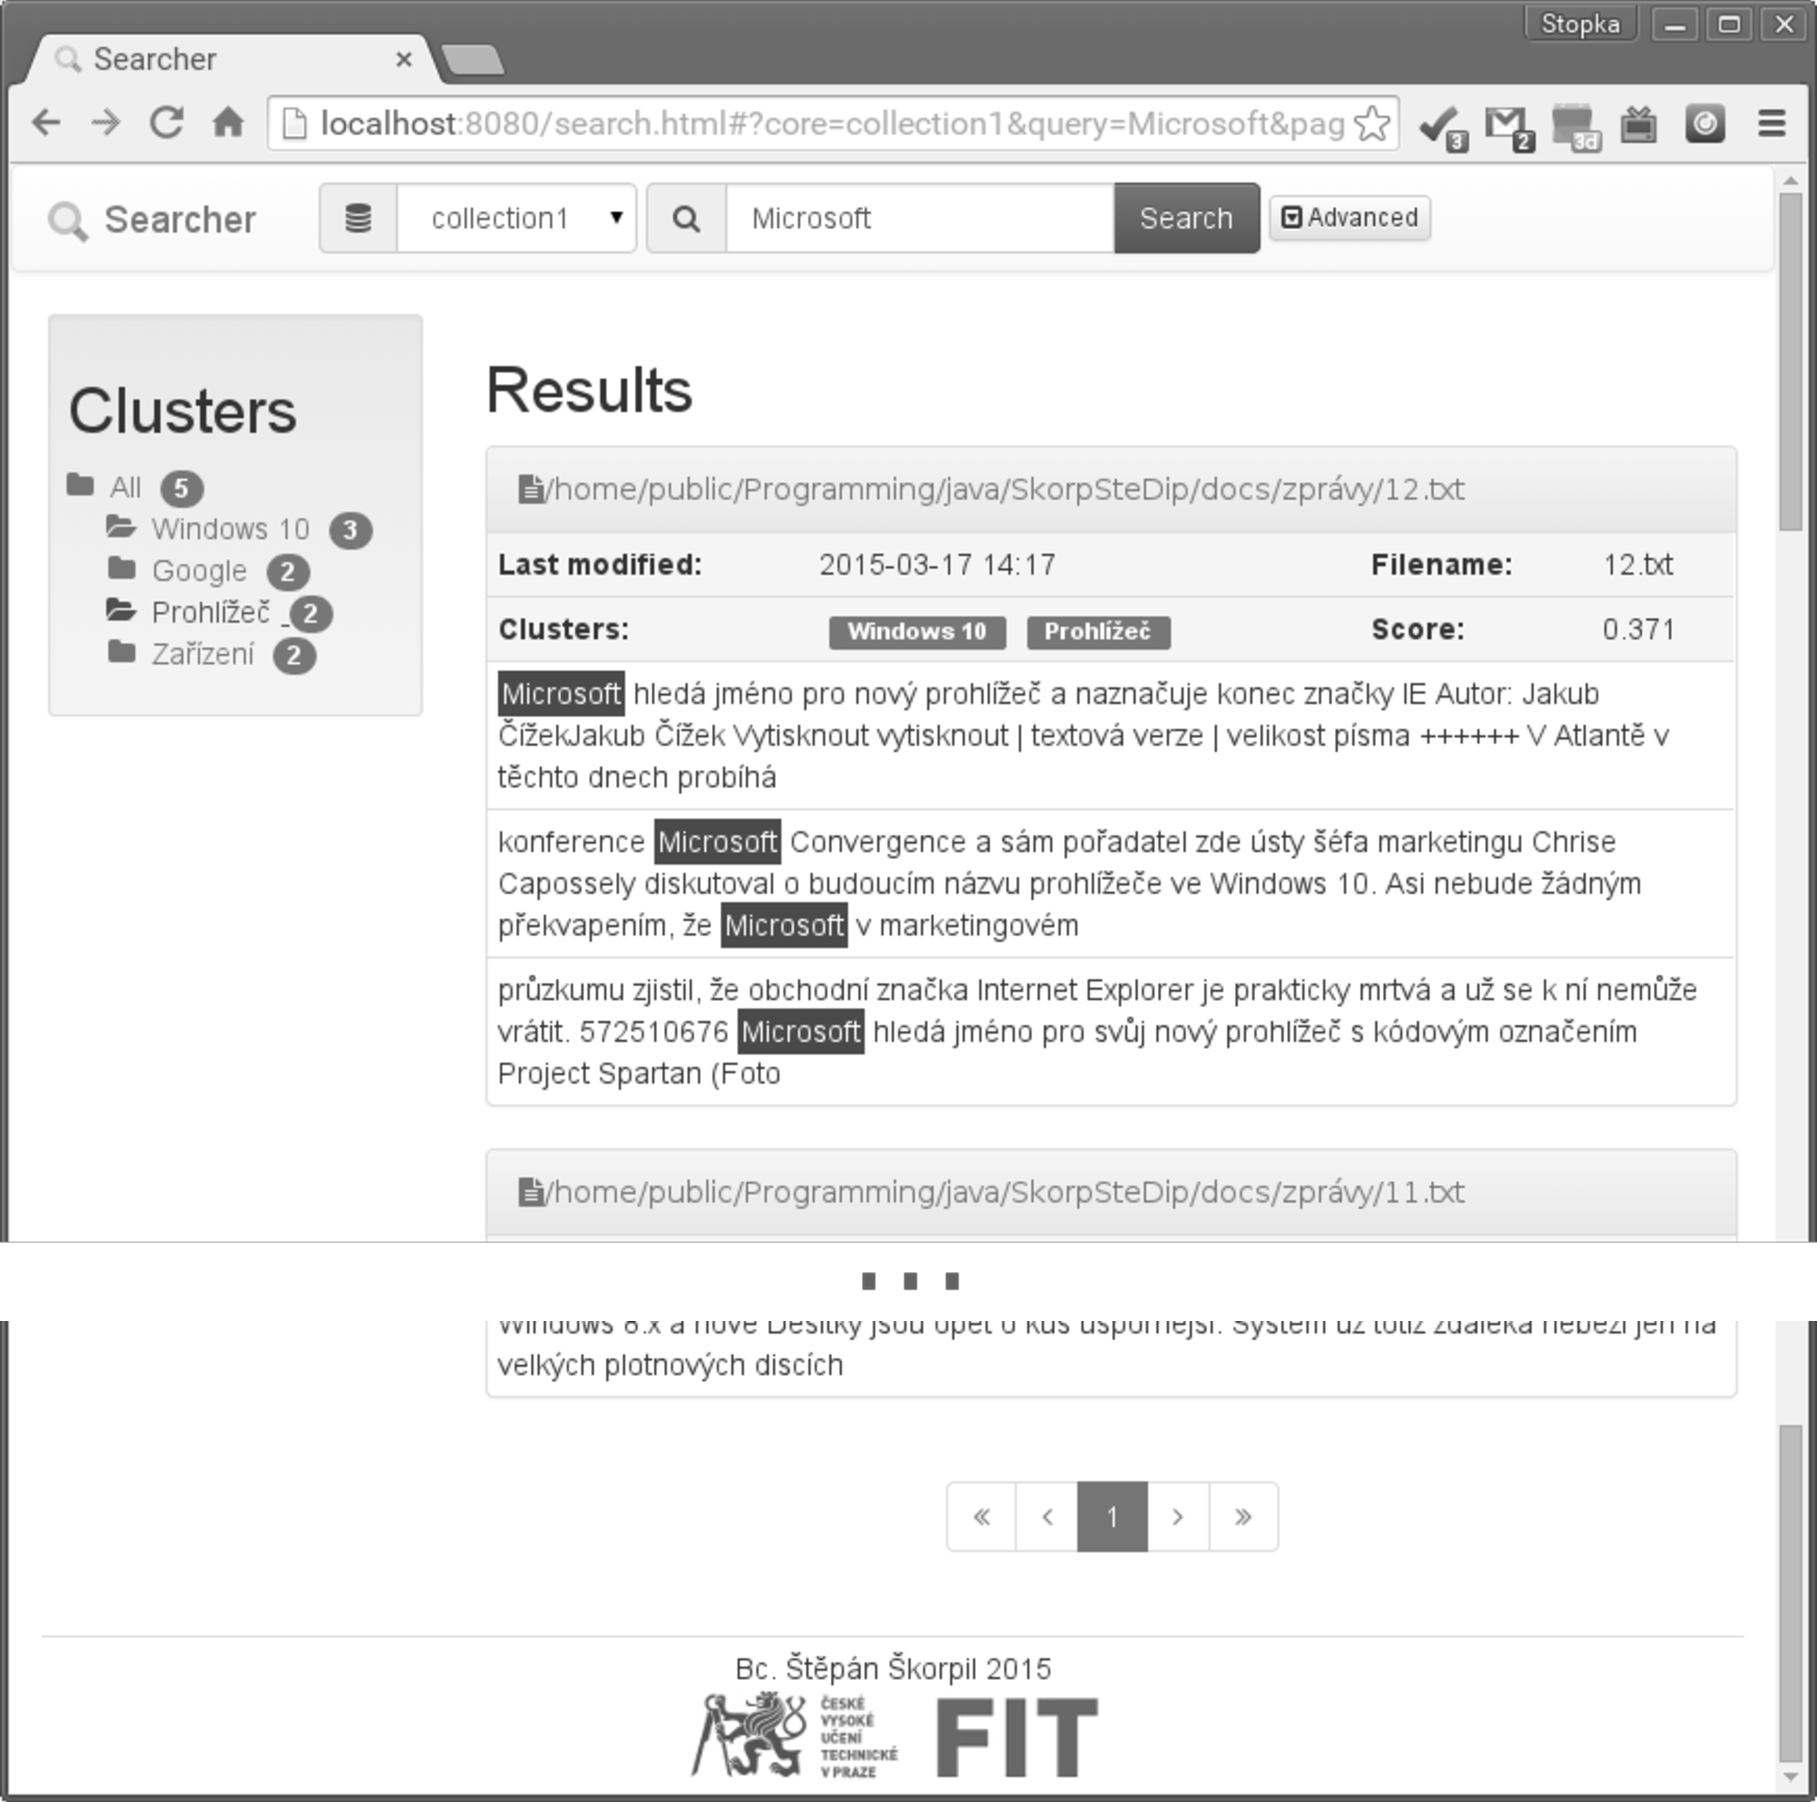
\includegraphics[width=13cm]{ScreenSearcher}
\caption{Snímek UI (Vyhledávač)}
\label{fig:ScreenSearcher}
\end{center}
\end{figure}

\begin{figure}[h]
\begin{center}
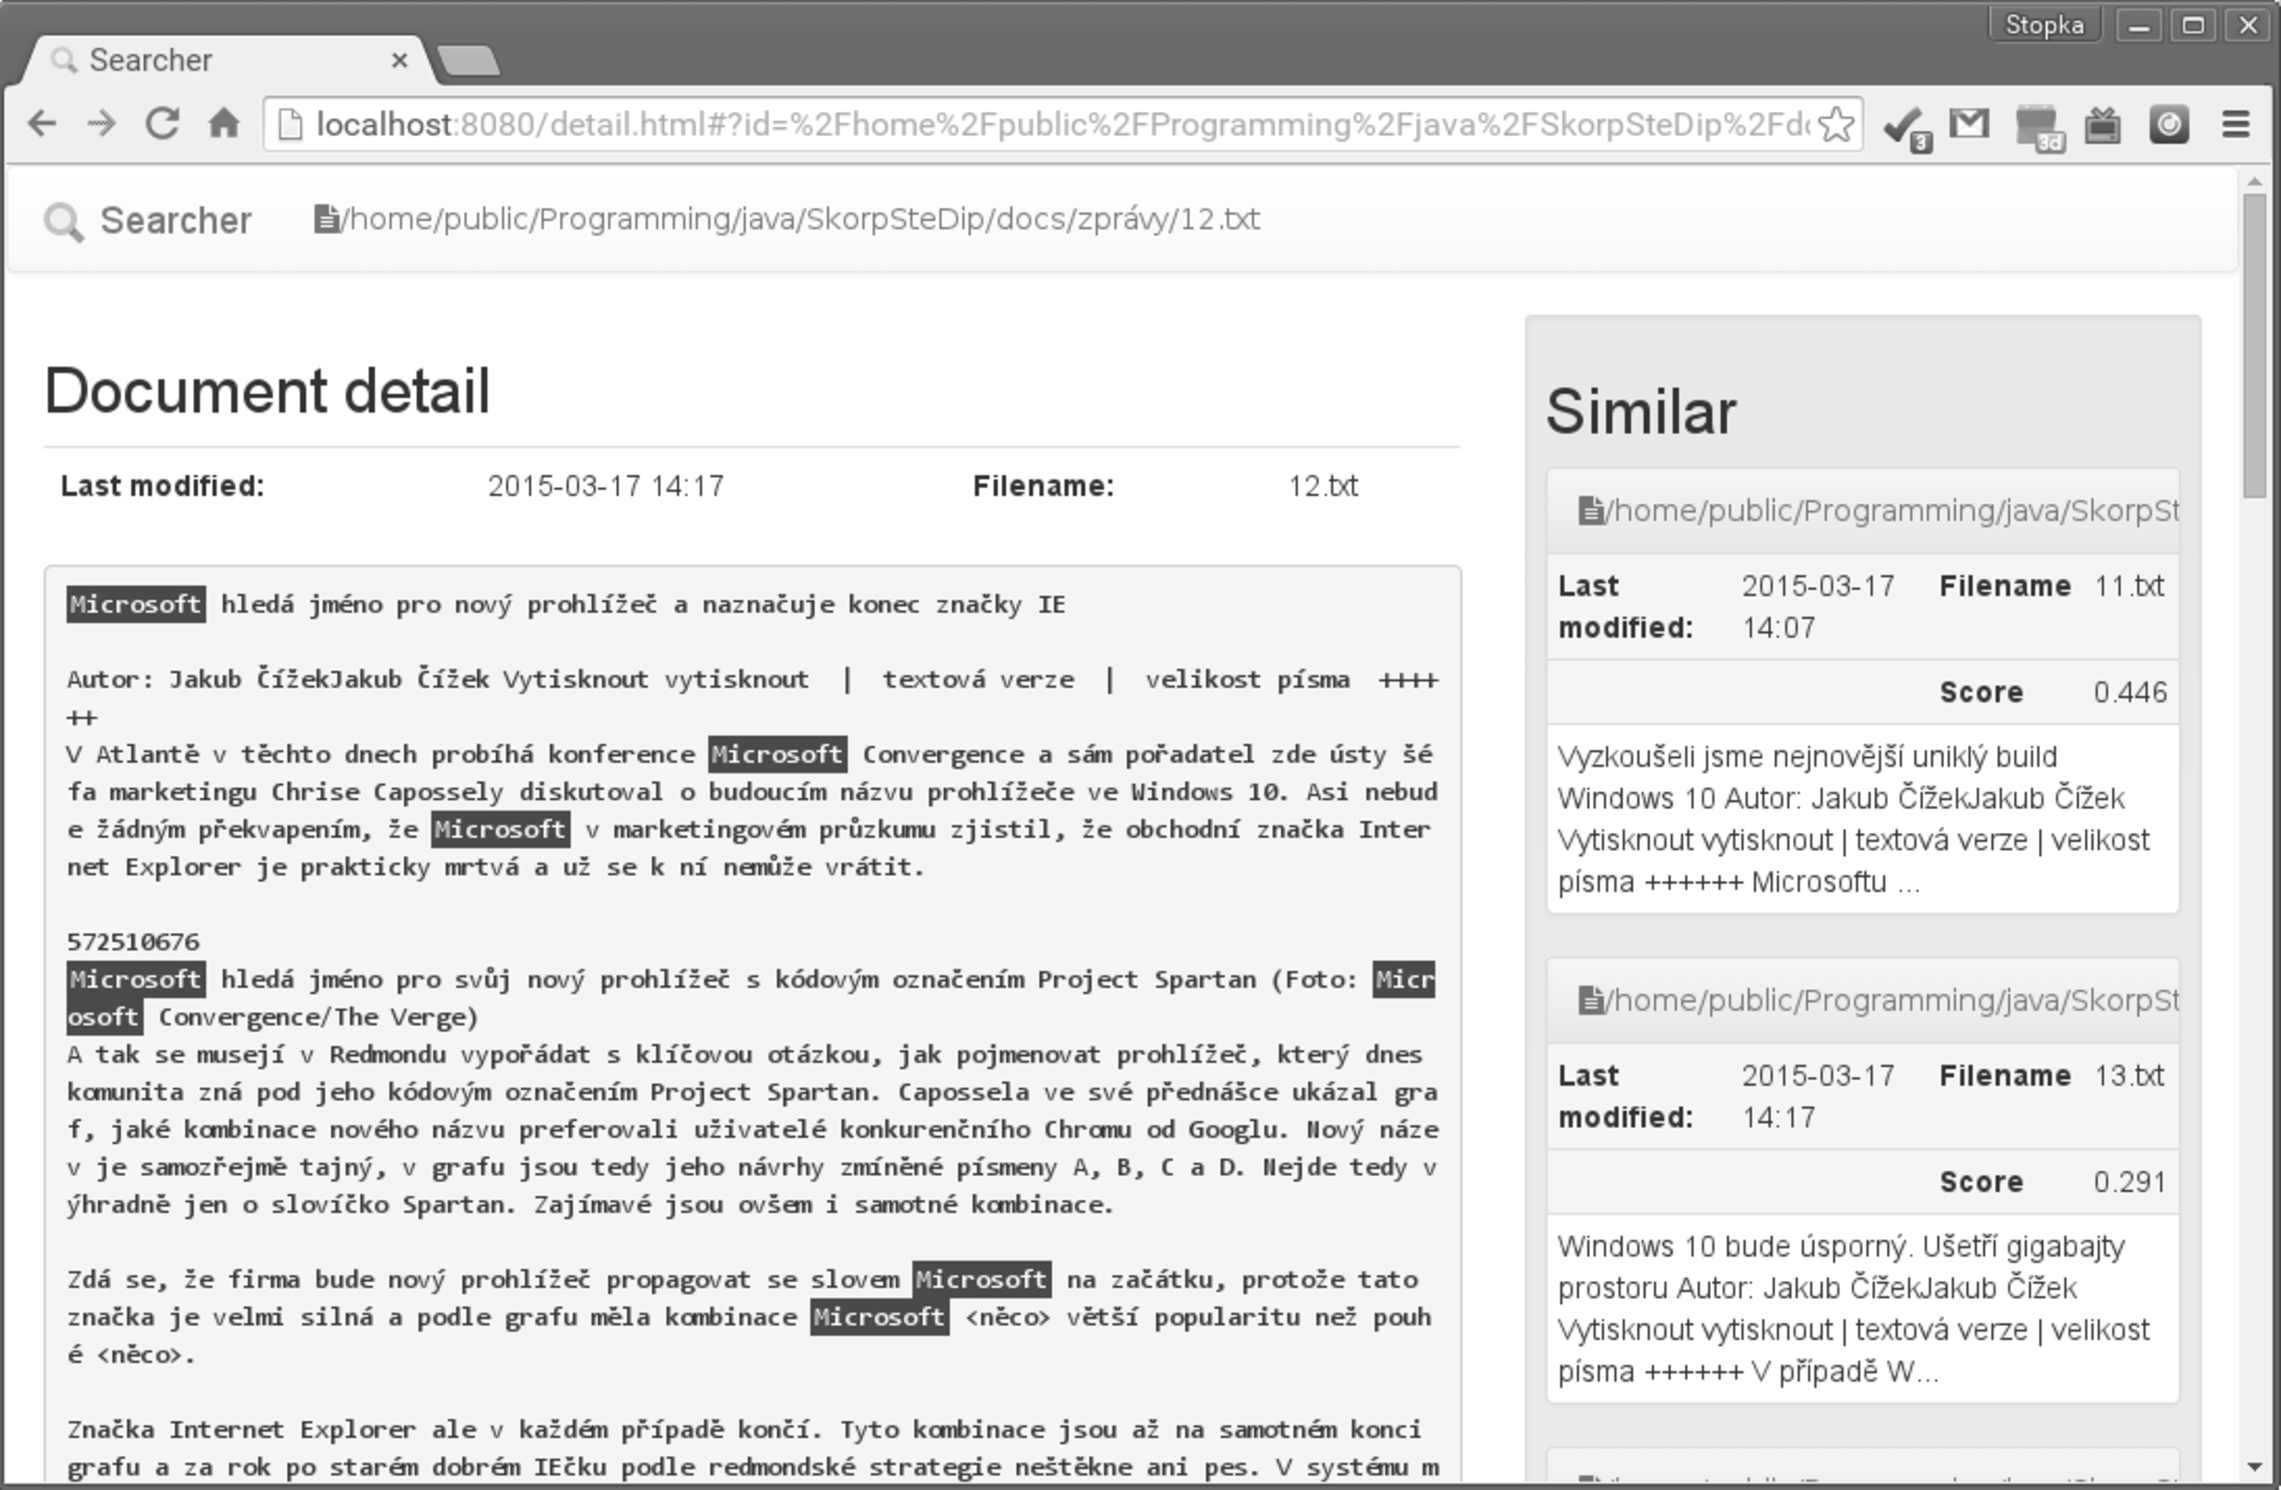
\includegraphics[width=13cm]{ScreenDetail}
\caption{Snímek UI (Detail dokumentu)}
\label{fig:ScreenDetail}
\end{center}
\end{figure}
\chapter{Testování} \label{testing}
\section{Test stemmerů}
\subsection{Správnost kořenů}
Tato část je věnována testování kvality jednotlivých implementovaných stemmerů. Helebrand pro účely testování svého stemmeru vytvořil seznamy slov, ve kterých ručně označil správné kořeny. V seznamu jsou u slov uvedeny dva kořeny, jeden lingvisticky naprosto správný, druhý méně správný, ale uznatelný tvar.

Seznamy jsou připraveny dva. Jeden obsahuje slova vybraná z reálného článku a umožní otestovat nasazení algoritmu v reálném prostředí. Druhý seznam slov je připravený speciálně pro otestování správné funkce stemmerů pro různé tvary slov včetně méně obvyklých tvarů a vyjímek. Obsažená slova jsou uvedena ve všech pádech a číslech. Slova jsou v seznamech tříděna do souborů podle slovních druhů, z~výsledků tedy bude možné odvodit úspěšnost získávání kořene slova jednotlivých slovních druhů.

V jazyce Ruby jsem naprogramoval krátký jednoúčelový skript, který na základě parametrů načte příslušný seznam slov a zparsuje výchozí tvary slov a jejich označené kořeny. Jednotlivá slova pak nechá převést na jejich kořeny analyzerem s příslušným stemmerem tak, že je přímo pošle na REST rozhraní Solru. Získaný kořen pak porovná s~označenými kořeny v~seznamu. Průběžné výsledky zapíše do výstupního souboru, aby bylo možné provádět hlubší analýzy. Nakonec skript zobrazí a  do výstupního souboru zapíše číselné hodnoty, které odpovídají celkovému počtu slov a~počtu slov, která byla stemována na žádaný tvar. Tímto způsobem lze vyjádřit procentuální úspěšnost algoritmu.

Pomocí tohoto skriptu jsem otestoval všechny implementované české stemmery. Výsledky jsou uvedeny v~tabulce \ref{tab:test_stm}. Z~ní také můžeme vyčíst, že v~tomto testu si vede nejhůře původní stemmer. Nejlépe pak dopadl Helebrand stemmer. Výsledky testu rovněž prokázaly, že slovníkový stemmer Hunspell není celkově příliš účinný, ale má velmi dobré výsledky v kategorii sloves --- pravděpodobně proto, že jde spíše o~lematizer, který vrací slova v~základním tvaru, takže se utvořený tvar neshoduje s~označným kořenem. Malá účinnost je zároveň důsledkem nízké kvality českého slovníku, neboť je třeba brát v potaz, že v době jejich vzniku byly určeny ke kontrole pravopisu.

V rámci další analýzy výsledků algoritmů jsem procházel výstupní soubory s vytvořenými kořeny a zjistil jsem, že nenalezne-li Hunspell slovo ve slovníku, vrací původní tvar slova. Napadlo mě tedy zkusit spojit dva stemmery za sebe. Slovo by se nejdříve předložilo Hunspell stemmeru. Kdyby nebyl úspěšný, slovo by zůstalo v původním tvaru a je možné jej předložit stemmeru dalšímu. Když bude úspěšný, vrátí slovo v základním tvaru podle slovníku a další stemmer v pořadí bude mít jednodušší práci s ořezáním slova na jeho kořen. V obou případech by měl být výsledkem kořen slova použitelný pro indexaci. V konfiguraci Solru jsem tedy vytvořil další analyzer obsahující dva stemmery. Jako druhý stemmer po slovníkovém jsem zvolil ten, který měl v testu nejlepší výsledek --- Helebrandův.

Výsledný analyzer jsem otestoval stejným způsobem jako předešlé a~zanesl výsledek do tabulky \ref{tab:test_stm} pod názvem \emph{text\_cz\_hh}. Analyzer dosáhl rekordní úspěšnosti 70,98\%. Obě metody se dle očekávání doplňují. Slovník přispívá vysokou přesností, druhý stemmer možností univerzálního použití pro kterékoliv slovo.

\begin{table}
\begin{center}
\begin{tabular}{|l|r|r|r|r|r|r|r|r|}
\hline
(\%) & \multicolumn{2}{|c|}{\textbf{Podst. jm.}} & \multicolumn{2}{|c|}{\textbf{Příd. jm.}} & \multicolumn{2}{|c|}{\textbf{Slovesa}} & \multicolumn{2}{|c|}{\textbf{Vše}} \\ \hline
\textbf{Stemmery} & \textbf{Čl.} & \textbf{Tst.} & \textbf{Čl.} & \textbf{Tst.} & \textbf{Čl.} & \textbf{Tst.} & \textbf{Čl.} & \textbf{Tst.} \\ \hline
cz & 51,68 & 3,07 & 39,69 & 4,15 & 7,58 & 2,44 & 38,50 & 3,20 \\ \hline
cz\_light & 60,40 & 3,80 & 46,56 & 2,63 & 11,36 & 2,64 & 45,63 & 3,40 \\ \hline
cz\_agressive & 55,03 & 48,53 & 52,67 & 23,37 & 3,03 & 0,00 & 42,25 & 36,61 \\ \hline
cz\_helebrand & 53,69 & 58,47 & 49,62 & 47,16 & 31,82 & 38,62 & 47,59 & 53,39 \\ \hline
cz\_hunspell & 35,91 & 0,00 & 1,53 & 0,00 & 70,45 & 90,04 & 38,04 & 12,55 \\ \hline
\hline
cz\_hh & 56,04 & 74,42 & 54,20 & 66,39 & 39,39 & 61,59 & 51,69 & 70,98 \\ \hline
\end{tabular}
\end{center}
\caption{Výsledek testu správnosti kořenů}
\label{tab:test_stm}
\end{table}

\subsection{Shodnost kořenů}
Po další důkladné analýze výsledků předchozího testu jsem zjistil, že test nevypovídá dostatečně o vhodnosti nasazení stemmeru pro indexaci a~vyhledávání. Pro nejlepší výsledky je nutné, aby stemmer tvořil pokud možno stejný kořen pro všechny tvary jednoho slova, což se v~mnoha případech nedělo.

Připravil jsem tedy test nový. Odvodil jsem nový seznam slov, kde na řádku jsou vždy uvedeny různé tvary téhož slova. Upravil jsem také testovací algoritmus, který tentokrát postupně nechá všechny tvary jednoho slova  zpracovat analyzerem Solru a porovná vytvořené kořeny mezi sebou. Poté spočítá, kolik procent kořenů se shoduje. Čím více slov se tedy zpracuje do stejného kořene, tím vyšší číslo a tím lepší podal algoritmus výsledek na daném slově. Celkovou úspěšnost algoritmu odvozuji ze dvou čísel a to z průměrné úspěšnosti, získané aritmetickým průměrem úspěšnosti na jednotlivých slovech a úspěšnosti, počítané jako procento slov, u nichž se všechny tvary převedly na shodný tvar (jinými slovy na kolika procentech slov měl algoritmus stoprocentní úspěšnost).

Výsledky testu jsem můžeme pozorovat v tabulce \ref{tab:test_eql}. První sloupec udává pro daný slovní druh průměrný počet nalezených shodných kořenů, druhý pro kolik slov byl nalezen shodný kořen pro všechny jejich tvary. Tento test ukazuje, že nejlepších výsledků dosahuje slovníkový Hunspell stemmer. Druhým nejlepším je původní stemmer zabudovaný v Solru.

Oba stemmery předstihuje pouze kombinace Hunspell a Helebrnd stemmeru, vytvořená po minulém testu, což potvrzuje funkčnost navrženého principu kombinování. Protože jsou výsledky tohoto testu odlišné než výsledky testu předchozího, vytvořil jsem nový analyzer s použitím nejúspěšnějších stemmerů v nové testu --- Hunspell a původní stemmer. Nový kombinovaný analyzer jsem také podrobil testu a výsledky zanesl do tabulky pod jménem \emph{text\_cz\_hx}. Nově vytvořený stemmer dosahuje nejlepších výsledků a~zdá se tak být pro vyhledávání nejvhodnějším kandidátem.

V konfiguraci Solru jsem na základě výsledků testu nastavil pro pole \emph{text} datový typ \emph{text\_cz\_hx} sestávající z~po sobě jdoucích \emph{solr.Hunspell} stemmeru a~\emph{solr.CzechStemmer}.

\begin{table}
\begin{center}
\begin{tabular}{|l|r|r|r|r|r|r|r|r|}
\hline
(\%) & \multicolumn{2}{|c|}{\textbf{Podst. jm.}} & \multicolumn{2}{|c|}{\textbf{Příd. jm.}} & \multicolumn{2}{|c|}{\textbf{Slovesa}} & \multicolumn{2}{|c|}{\textbf{Vše}} \\ \hline
\textbf{Stemmery} & \textbf{Pr.} & \textbf{Úsp.} & \textbf{Pr.} & \textbf{Úsp.} & \textbf{Pr.} & \textbf{Úsp.} & \textbf{Pr.} & \textbf{Úsp.} \\ \hline
cz & 98,38 & 92,00 & 94,60 & 40,00 & 24,95 & 1,82 & 85,09 & 62,22 \\ \hline
cz\_light & 87,40 & 38,00 & 81,38 & 3,64 & 23,50 & 1,52 & 75,08 & 21,11 \\ \hline
cz\_agressive & 89,57 & 54,00 & 91,75 & 31,64 & 39,35 & 1,82 & 81,81 & 37,78 \\ \hline
cz\_helebrand & 77,91 & 33,27 & 59,92 & 3,27 & 52,27 & 5,15 & 68,64 & 18,48 \\ \hline
cz\_hunspell & 86,66 & 44,18 & 84,10 & 32,00 & 94,39 & 66,67 & 87,24 & 44,55 \\ \hline
\hline
cz\_hh & 90,44 & 51,09 & 90,00 & 32,00 & 94,39 & 66,67 & 90,97 & 48,38 \\ \hline
cz\_hx & 97,05 & 89,82 & 94,60 & 40,00 & 94,39 & 66,67 & 95,92 & 72,12 \\ \hline
\end{tabular}
\end{center}
\caption{Výsledek testu shody kořenů}
\label{tab:test_eql}
\end{table}

\section{JUnit}
Všechny zásadní celky kódu jsou pokryty testy, které kontrolují integritu komponent pomocí \emph{JUnit}. Testy budou užitečné při případném dalším rozšiřování. Pokud dojde budoucí úpravou k~nechtěné zásadní změně funkčnosti existujících komponent, měly by to testy odhalit.

V~aplikaci Crawler jsou takto pokryty všechny procesorové komponenty a~crawlery. V~rozšiřující Solr knihovně \emph{Analyzery.jar} jsou pokryty všechny tři nové stemmery i~s~jejich továrními třídami.

Všechny napsané testy aktuálně hlásí stoprocentní úspěšnost.

\section{Test použitelnosti}
V tomto testu byla aplikace předložena skutečným uživatelům, aby otestovali navržené uživatelské rozhraní. Ověřím tak intuitivnost a funkčnost návrhu i imeplementace.

\subsection{Výběr uživatelů}
Testovací uživatele jsem volil především podle kritéria zkušenosti s prací s internetovými vyhledávači. Vybral jsem uživatele, kteří se běžně pohybují na internetu, umějí ovládat internetový prohlížeč, mají zažité zvyklosti z tohoto prostředí a běžně vyhledávají informace pomocí internetových vyhledávačů. Toto kritérium by mělo přesně vymezit skupinu uživatelů, pro kterou bylo uživatelské rozhraní určeno.

Uživatele jsem se rozhodl vybírat z okruhu svých přátel a to z několika důvodů. Jednak u nich mám představu o úrovni jejich znalostí a schopností, tudíž si mohu zvolit takové testovací uživatele, kteří spadají do výše zmíněné cílové skupiny. Takoví uživatelé ke mně budou během provádění testu také více otevření, tudíž se dozvím s menším úsilím více detailů o problémech, se kterými se potýkali.

\subsection{Charakteristika uživatelů}
Uživatelka Karolína je studentkou Filozofické fakulty Univerzity Karlovy. Počítač využívá k tvorbě školních prací, k práci s internetem, komunikaci i sledování multimédií. Je schopná na počítači provést i některé složitější konfigurační úkony, její uživatelské schopnosti tak hodnotím jako vysoké. Na internetu se pohybuje každodenně, často hledá informace skrze internetové služby, sleduje video portály, navštěvuje sociální sítě. Taktéž její zkušenost s internet hodnotím jako vysokou.

Uživatelka Petra používá počítač pro prohlížení a zálohu fotografií, práci s dokumenty a práci na internetu. Konfigurační úkony jsou pro ni velkou neznámou. Na internetu využívá sociální sítě, e-mailové služby, zpravodajské weby a vyhledávače. Web používá i k prodeji a propagaci zboží. Její počítačové schopnosti jsem tedy vyhodnotil spíše jako průměrné, internetové jako vysoké.

Uživatel Miroslav je absolventem Strojní fakulty ČVUT, jeho počítačové zkušenosti považuji za průměrné. Počítač používá pouze pro psaní dokumentů a k práci na internetu. Internet používá převážně k e-mailové komunikaci. Informace na internetu vyhledává v porovnání s předchozími uživatelkami méně často.

Anna je studentkou Ústavu translatologie na Filozofické fakultě Univerzity Karlovy. Počítač používá pro plnění školních povinností i pro zábavu. Na internetu používá sociální sítě, e-mailové služby, zpravodajské weby i vyhledávání. Ve vyhledávání na internetu je velmi pokročilá, denně při překladu vyhledává správná užití frází pomocí pokročilých technik dotazování internetových vyhledávačů.

Posledním uživatelem, který se účastnil testu, je Vladimír. Vladimír je studentem Technické univerzity v Liberci. V testu je nejpokročilejším uživatelem. Ve volném čase se zabývá programováním webových stránek i složitějších aplikací.

Základní orientační charakteristiku vybraných uživatelů znázorňuje tabulka \ref{tab:test_usrs}.

\begin{table}
\begin{center}
\begin{tabular}{|l|l|l|l|l|l|}
\hline
\textbf{Jméno} & \textbf{Věk} & \textbf{Pohlaví} & \textbf{Vzdělání} & \textbf{PC gram.} & \textbf{WWW gram.} \\ \hline
Karolína & 21 & Žena & Maturita & Vysoká & Vysoká \\ \hline
Petra & 46 & Žena & Maturita & Průměrná & Vysoká \\ \hline
Ing. Miroslav & 54 & Muž & Vysokoškolské & Průměrná & Průměrná \\ \hline
Anna & 21 & Žena & Maturita & Vysoká & Vysoká \\ \hline
Vladimír & 20 & Muž & Maturita & Expertní & Expertní \\ \hline
\end{tabular}
\end{center}
\caption{Testovací uživatelé}
\label{tab:test_usrs}
\end{table}

\subsection{Průběh testu}
Testovacím uživatelům jsem stručně představil aplikaci, seznámil jsem je s účelem aplikace, v bodech jsem vyjmenoval možnosti, které nabízí, a vysvětlil jsem jim základní terminologii. Z celého průběh testu jsem se svolením uživatelů pořídil videonahrávku, abych mohl test zpětně analyzovat a vyvodit závěry. Test jsem prováděl s každým uživatelem zvlášť.

Do systému jsem pro účely testu nahrál data --- do jednoho indexu dokumenty s uloženými články z technického zpravodajského webu, do druhého anonymizované příklady policejních dokumentů. Uživatele jsem nechal několik minut zkoumat prostředí, aby se sami zběžně seznámili s funkcemi. Poté jsem uživatelům zadal následující úkoly a instruoval je, aby své kroky, nahlas komentovali. Během plnění úkolu jsem nezasahoval, pouze jsem pasivně pozoroval jejich počínání.

\begin{enumerate}
\item Vyhledejte dokumenty týkající se firmy \uv{Microsoft}.
\item Zjistěte, jaké shluky se ve výsledcích vyskytují.
\item Zjistěte, v jakých shlucích se nachází první výsledek.
\item \label{task_clusterfilter}Odfiltrujte pouze výsledky ve shlucích \uv{Windows 10} a \uv{Google}.
\item Zobrazte z novu všechny výsledky hledání.
\item Otevřete první dokument ve výsledcích.
\item Otevřete dokument, který je otevřenému dokumentu nejpodobnější.
\item Vyhledejte v druhé kolekci dokumenty, které obsahují spojení \uv{úřední záznam}.
\item \label{task_engine}Změňte mechanismus shlukování.
\item Zjistěte, kdy byly nalezené dokumenty naposledy upraveny.
\end{enumerate}

Úkoly byly navrženy tak, aby prověřily především klíčové aspekty rozhraní, jako například zda uživatel bude vědět, jak se vrátit z detailu dokumentu, zda uživatel pochopí funkci filtrování podle shluků a zda pochopí možnost přepínání kolekcí či shlukovacích algoritmů.

Po dokončení testu jsem s každým uživatelem ještě diskutoval o návrzích na vylepšení a dotázal jsem se na jejich porozumění funkcím jednotlivých detailů prvků rozhraní. Zaměřil jsem se na následující body.

\begin{itemize}
\item Jestli vědí, co vyjadřuje číslo u každého shluku.
\item Jestli bezpečně rozeznají otevřené shluky.
\item Jestli dokáží zjistit, do jakých shluků dokument patří.
\item Jestli vědí, jaké výsledky se zobrazují ve výchozím stavu.
\item Jestli rozumí metadatům dokumentu.
\end{itemize}

Po každém testu jsem vždy rovnou navrhl a implementoval řešení nalezených kritických problémů, abych v dalších testech ihned viděl, zda má opatření účinek.

\subsection{Výsledky testu}
\subsubsection{Karolína}
Jako první jsem test provedl s uživatelkou Karolínou. Uživatelka neměla problém s rozeznáním funkcí uživatelského rozhraní. Největší problém nastal v bodě \ref{task_clusterfilter}, kde měla vybrat výsledky jen z daných shluků. Uživatelku nenapadlo kliknout na více shluků a tím jich více vybrat. V následné diskusi jsem zjistil, že se tak stalo kvůli nedostatečným zvýrazněním otevřených shluků. Otevřený shluk nyní změní pouze přidruženou ikonu složky z běžné na otevřenou, což uživatelka nepostřehla, nebo nebrala v úvahu. Zároveň jí zmátlo barevné označení odkazu po kliknutí. Prohlížeč Chrome totiž neodebírá správně \emph{hover} efekt odkazu po odjetí myši z odkazu.

Na základě tohoto poznatku jsem dodatečně provedl drobnou úpravu frontendu. Řádek s otevřeným shlukem se označí nejen ikonou otevřeného adresáře, ale i změnou barvy. Tím by mělo dojít k dostatečnému zvýraznění otevřených shluků.

\subsubsection{Petra}
Následně jsem test provedl s uživatelkou Petrou. Ta se v prostředí také rychle zorientovala. Problém nastal opět u úkolu \ref{task_clusterfilter}. Aktuální vizualizace otevřeného shluku stále dostatečně nenapovídá, že lze filtrovat výsledky podle více shluků.

Další problém nastal v bodě \ref{task_engine}. Možnost přepnout shlukovací algoritmus hledala v prostoru bloku s nalezenými shluky a vůbec ji nenapadlo otevřít rozšířenou nabídku vyhledávání. Nabídku jsem dle zvyklostí z jiných vyhledávačů umístil vpravo od vyhledávacího pole. Rozšířenou nabídku uživatelka nepoužívá ani v běžných internetových vyhledávačích. Tento úkon naštěstí není nutný pro běžné vyhledávání, proto je nabídka běžně schovaná a proto také není velkým problémem, když ji uživatel hned nenajde. 

Diskuzí jsme nakonec dospěli ještě k jedné nesrovnalosti. Při vyhledávání je každý výsledek zobrazen se třemi úryvky textu, ve kterých jsou zvýrazněna vyhledávaná slova. Každý úryvek je oddělen vizuálně novým řádkem tabulky a to se zdálo být matoucí.

Na základě výsledků tohoto testu jsem opět vyvodil drobné změny v návrhu UI. Znovu jsem opravil zvýraznění otevřených shluků v seznamu a nahradil původní ikonu otevřeného či zavřeného adresáře ikonou zaškrtnutého či nezaškrtnutého formulářového políčka \emph{checkbox}. Uživatelé jsou zvyklí z formulářů na internetu, že zaškrtávací pole ve tvaru čtverce znamenají možnost vybrat více položek, tato úprava by by jim tedy měla napovědět i v tomto případě.

Dále jsem se pokusil řešit problém s úryvky textu ve výsledcích. Existují dvě možnosti. Buď se zobrazí jen jeden delší úryvek, nebo se změní způsob zobrazení úryvků tak, aby byly méně matoucí. Rozhodl jsem se pro druhou možnost. Nadále se budou zobrazovat tři úryvky, neboť mi připadá výhodné zobrazit více relevantního textu s hledanými slovy, což pak usnadní hledání požadovaného dokumentu. Změní se však způsob zobrazení úryvků. Úryvky se nebudou zobrazovat ve třech samostatných řádcích, ale budou v jednom bloku odděleny obyčejnou textovou výpustkou.

\subsection{Ing. Miroslav}
Miroslav měl s použitím softwaru největší potíže. Největší problém představovalo najít schovanou nabídku přepínání shlukovacího algoritmu. Hledal ji spíše v místě nabídky kolekcí, ale nakonec ji úspěšně našel. Navíc očekával, že změna algoritmu proběhne ihned při změně ve vstupním poli, a byl zmaten, když se tak nestalo.

Miroslav si také nebyl jistý funkcí filtrování podle shluků. Ihned ale pochopil, že může zaškrtnout i více položek, takže předchozí opravná opatření se zdají být úspěšná. Nebyl si však jistý jak se výsledek filtrování projevil. Nepostřehl, že se mezi výsledky zobrazují jen některé dokumenty. Rozhodl jsem se tedy provést ještě jednu drobnou změnu: u každé položky se zvýrazní barevně shluky, podle kterých se filtruje.

\subsection{Anna}
Anna zvládla všechny úkoly bez zjevného zaváhání. V následné diskuzi o proběhlém testu se pouze přiznala, že hned nevěděla, jak otevřít detail dokumentu. Zkoušela kliknout nejdříve na text dokumentu ve výsledcích, než si všimla, že je v hlavičce odkaz.

Zvažoval jsem, že bych jako odkaz na detail dokumentu označil celý box patřící položce výsledku. Tuto možnost jsem však nakonec zavrhl. Uživatelé by například mohli mít potíže s kopírováním textů a podobně.

\subsection{Vladimír}
Poslední test jsem provedl s uživatelem Vladimírem, přičemž s jeho zkušenostmi by se tento test dal označit spíše za expertní test. Uživatel neměl s použitím aplikace žádný větší problém. Jeho jedinou drobnou připomínkou bylo, že na stránce s detailem dokumentu hledal tlačítko pro návrat, než si uvědomil, že může použít funkce prohlížeče.

\section{Akceptační test}
Posledním provedeným testem byl akceptační test. Prošel jsem jednotlivé definované požadavky na systém a~ověřil jejich splnění. Všechny požadavky, které jsem zařadil do první fáze projektu a~kterým se věnuje tato práce jsou splněny. Ostatní požadavky jsou odloženy, jelikož nebylo v~mých silách implementovat celé tak rozsáhlé zadání. Detailní rozpis je uveden v~tabulce \ref{tab:test_accept}.
\begin{table}
\begin{center}
\begin{tabular}{|l|l|p{6cm}|}
\hline
\multicolumn{3}{|c|}{\textbf{\ref{req_0} Funkční požadavky}} \\ \hline
\multicolumn{2}{|l|}{\textbf{Požadavek}} & \textbf{Stav} \\ \hline
\ref{req_00} & Indexace textových souborů & Splněno\\ \hline 
\ref{req_01} & Rozšíření o~další index dokumentů & Splněno\\ \hline 
\ref{req_02} & Ukládání celého obsahu dokumentů & Splněno\\ \hline 
\ref{req_03} & Zpracovávání textu v~českém jazyce & Splněno\\ \hline 
\ref{req_04} & Fulltextové vyhledávání v~dokumentech & Splněno\\ \hline 
\ref{req_040} & Tokenizace českého textu & Splněno\\ \hline 
\ref{req_041} & Stemizace českého textu & Splněno\\ \hline 
\ref{req_042} & Zobrazení obsahu nalezených dokumentů & Splněno\\ \hline 
\ref{req_043} & Zvýraznění hledaných slov & Splněno\\ \hline 
\ref{req_05} & Zobrazení podobných dokumentů & Splněno\\ \hline 
\ref{req_050} & Počítání podobnosti dokumentů & Splněno\\ \hline 
\ref{req_06} & Shlukování výsledků hledání & Splněno\\ \hline 
\ref{req_060} & Shlukování do automatických kategorií & Splněno\\ \hline 
\ref{req_061} & Filtrování výsledků podle shluků & Splněno\\ \hline 
\ref{req_07} & Rozpoznávání jmenných entit & Odloženo do dalších fází\\ \hline 
\ref{req_070} & Rozpoznávání větných členů & Odloženo do dalších fází\\ \hline 
\ref{req_071} & Rozpoznávání slovních druhů & Odloženo do dalších fází\\ \hline 
\ref{req_072} & Porovnávání s~jmennými databázemi & Odloženo do dalších fází\\ \hline 
\ref{req_08} & Extrakce vazeb mezi entitami & Odloženo do dalších fází\\ \hline 
\hline
\multicolumn{3}{|c|}{\textbf{\ref{req_1} Nefunkční požadavky}} \\ \hline
\multicolumn{2}{|l|}{\textbf{Požadavek}} & \textbf{Stav} \\ \hline
\ref{req_10} & Čistě open source technologie & Splněno\\ \hline 
\ref{req_11} & Architektura klient-server jako webová služba & Splněno\\ \hline
\ref{req_12} & Nativně nasaditelný pod Windows & Splněno\\ \hline
\ref{req_13} & Rozšiřitelnost & Splněno\\ \hline
\end{tabular}
\end{center}
\caption{Výsledek akceptačního testu}
\label{tab:test_accept}
\end{table}
\begin{conclusion}
Podařilo se mi navrhnout a implementovat systém, který dokáže spolehlivě vyhledávat a shlukovat české textové dokumenty vyšetřovatelů. Jedná se zatím pouze o první část navrženého komplexního řešení, které by vyšetřovatelé potřebovali. K dalším částem bude zapotřebí integrovat další, ještě pokročilejší metody zpracování textu.

V práci jsem využil pouze open source technologie, především aplikace Solr a Carrot2, do kterých jsem implementoval nové nástroje pro zpracování českých textů. Speciálně jsem se zaměřil na nástroje pro získání kořenů slov, takzvané stemmery. Kvality těchto nástrojů jsem otestoval a vybral ty nejvhodnější pro účely vyhledávání v textu. 

Mnou navržený český stemmer (respektive kombinace stemmerů) je dle mých testů o deset procent úspěšnější než původní stemmer obsažený v Solru. K tomu jsem navíc implementoval i další stemmery, z nichž jeden má vysokou úspěšnost tvorby správných lingvistických kořenů, což může být využito v dalších fázích implementace budoucího řešení zpracování textu.

K dosažení všech definovaných cílů jsem vytvořil několik přidružených aplikací, například \emph{Crawler}, aplikace, která se k Solru připojuje a která má za úkol přidávání a odebírání dokumentů z indexu. Aplikaci se mi podařilo navrhnout plně modulární a tedy i do budoucna rozšiřitelnou.

Pro Solr jsem také vytvořil webový frontend pro uživatelské vyhledávání v dokumentech, postavený na moderních technologiích jako HTML5, CSS3 či Angular.js. Frontend je navržený s důrazem na intuitivnost, což bylo ověřeno uživatelským testováním.

Výsledný systém jsem se snažil koncipovat tak, aby mohl být dále rozšiřován o další moduly či aplikace tak, aby v dalších fázích projektu mohlo být na tuto implementovanou část navázáno. Tomu jsem podřídil výběr technologií i dalších prostředků vývoje.

Po celou dobu vývoje jsem své kroky konzultoval se zadavatelem projektu, aby výsledek co nejvíce vyhovoval jeho potřebám. I tak už nyní vyvstávají nové návrhy, jak aplikaci pro vyhledávání ještě dále vylepšit. Zadavatel by například uvítal možnost vyhledat dokumenty i z několika kolekcí (myšleno indexů) naráz. Technicky by nový požadavek mohl být splněn například úpravou frontendu, který by dotaz rozeslal do vybraných kolekcí a výsledky sloučil. Tato možnost poměrně jednoduchého řešení dodatečných požadavků pouze úspěšně dokazuje rozšiřitelnost návrhu řešení.
\end{conclusion}

\bibliographystyle{csn690}
\bibliography{bibliography}

\appendix
\chapter{Seznam použitých zkratek}
% \printglossaries
\begin{description}
	\item[AJAX] Asynchronous JavaScript and XML
	\item[API] Application programming interface
	\item[CSS] Cascading Style Sheets
	\item[ČVUT] České Vysoké Učení Technické V~Praze
	\item[DOM] Document object model
	\item[HTML] Hypertext Markup Language
	\item[HTTP] Hypertext Transfer Protocol
	\item[ID] Identifikátor
	\item[JAR] Java archive
	\item[Java EE]	Java Platform, Enterprise Edition
	\item[JSON] JavaScript Object Notation
	\item[OBBB] Open Black Box Builder
	\item[PC] Personal Computer
	\item[REST] Representational State Transfer
	\item[STC] Suffix Tree Clustering
	\item[UI] User interface
	\item[URL] Uniform Resource Locator
	\item[XML] Extensible Markup Language
	\item[Java VM] Java Virtual Machine
	\item[WAR] Web application archive
	\item[WWW] World Wide Web
\end{description}
\chapter{Uživatelská příručka}
\section{Požadavky}
Systém ke svému běhu potřebuje následující softwarové prerekvizity. Aplikace může fungovat i na jiných verzích, na těchto zde napsaných byla aplikace testována.
\begin{itemize}
\item Windows 7/8; Linux 4
\item Java runtime 1.8 (na počítači \emph{search~server} a \emph{file~client}, viz kapitola\ref{arch})
\item Internetový prohlížeč Chrome~42/Firefox~37 (na počítači \emph{search~client}, viz kapitola \ref{arch})
\item Apache~Maven~3 (pouze pro kompilaci)
\item IntelliJ~Idea (doporučeno, pouze pro kompilaci)
\end{itemize}

\section{Instalace}
\begin{enumerate}
\item Zkopírujte adresář s aplikací \emph{searcher} do adresáře cílového počítače (\emph{search~server} - viz kapitola \ref{arch}).
\item Zkopírujte adresář s aplikací \emph{crawler} do adresáře cílového počítače (\emph{file~client} - viz kapitola \ref{arch})
\end{enumerate}

\section{Kompilace}
Kompilaci mají všechny součásti velmi podobnou, proto zde uvedu jednotný návod.
\begin{enumerate}
\item V~adresáři zdrojových souborů zavolejte program Maven příkazem \verb|maven clean build|.
\item Maven automaticky stáhne potřebné knihovny a sestaví knihovnu, webový archiv či java aplikaci. hotový archiv naleznete v~adresáři \emph{/target/} příslušné aplikace.
\end{enumerate} 

\subsection{Sestavení}
\begin{itemize}
\item Aplikace \emph{crawler} je samostatnou aplikací běžící v Java runtime. Všechny závislosti se při kompilaci přibalí do výsledného aplikačního archivu \emph{crawler-jar-with-dependencies.jar}
\item Knihovnu \emph{Analyzery} nainstalujete do solru zkopírováním výsledného souboru\emph{Analyzery.jar} do adresáře \emph{/searcher/solr/lib/} serverové aplikace.
\item \emph{Frontend} nainstalujete do solru zkopírováním výsledného souboru \emph{frontend.war} do adresáře \emph{/searcher/webapps/}.
\end{itemize}

\section{Searcher}
\subsection{Spuštění}
Aplikaci spustíte zavoláním skriptu \emph{run.bat} na Windows, respektive \emph{run.sh} na Linuxu. Po každé úpravě konfigurace je nutné aplikaci restartovat.

\subsection{Konfigurace}
\subsubsection{Změna portu}
Síťový port nastavíte v souboru \emph{/searcher/etc/jetty.xml} změnou hodnoty označené textem \emph{[PORT]} v následujícím úryvku. Ve výchozím stavu je port nastaven na \emph{8080}.
\begin{verbatim}
<Call name="addConnector">
  <Arg>
    <New class="org.eclipse.jetty.server.bio.SocketConnector">
      <Set name="port">
        <SystemProperty name="jetty.port" default="[PORT]"/>
      </Set>
    </New>
  </Arg>
</Call>
\end{verbatim}

\subsubsection{Přidání indexu}
Vytvořte kopii adresáře \emph{/searcher/solr/collection1} pro český index, nebo \emph{/searcher/solr/en\_collection1} pro anglický. Nový adresář vhodně pojmenujte, například \emph{/searcher/solr/collection2}. Upravte jméno kolekce změnou hodnoty \verb|name=collection2| v souboru \emph{/searcher/solr/collection2/core.properties}. Jméno kolekce musí být unikátní.

\subsubsection{Změna stemmeru}
Nahraďte \emph{[ANALYZER]} v úryvku souboru \emph{/searcher/solr/<kolekce>/conf/schema.xml} jménem analyzeru s požadovaným stemmerem.
\begin{verbatim}
<field name="text" type="[ANALYZER]" indexed="true" 
       stored="true" termVectors="true" />
\end{verbatim}
Přípustné hodnoty jsou \emph{text\_cz}, \emph{text\_cz\_light}, \emph{text\_cz\_agressive}, \emph{text\_cz\_helebrand}, \emph{text\_cz\_hunspell}, \emph{text\_cz\_hh}, \emph{text\_cz\_hx}. Výchozí hodnota je \emph{text\_cz\_hx}. Po změně je nutné přeindexovat všechny soubory.

\subsubsection{Změna výchozího shlukovacího algoritmu}
Nahraďte \emph{[ENGINE]} v úryvku souboru \emph{/searcher/solr/<kolekce>/conf/solrconfig.xml} jménem požadovaného shlukovacího enginu.
\begin{verbatim}
<requestHandler name="/searcher" startup="lazy"
                enable="${solr.clustering.enabled:false}"
                class="solr.SearchHandler">
  <lst name="defaults">
    <str  name="clustering.engine">[ENGINE]</str>
  </lst>
</requestHandler>
\end{verbatim}
Přípustné hodnoty jsou \emph{lingo} (výchozí), \emph{stc}, \emph{kmeans}.

\section{Crawler}
Crawler se spuští zavoláním skriptu \emph{run.bat} na Windows, respektive \emph{run.sh} na Linuxu. V rámci jednoho běhu se provedou dvě fáze: \emph{cleaning} a \emph{indexing}. \emph{Indexing} fáze prochází adresáře, hledá nové soubory a všechny soubory zanese do indexu. Existuje-li již soubor v indexu, aktualizuje jej. \emph{Cleaning} fáze projde všechny dokumenty v indexu a pokud již soubor neexistuje v adresáři, z indexu jej smaže. 

Veškerá konfigurace se provádí skrze konfigurační soubor či vstupní parametry. Ve výchozím stavu se hledá konfigurační soubor \emph{crawler.properties} v adresáři spuštění aplikace. Cesta ke konfiguračnímu souboru se může změnit přidáním parametru \emph{config}. Výsledný příkaz pro spuštění pak vypadá například následovně: \\ \verb|run.sh -Dconfig=cesta/k/souboru/nastavení.properties| \\

Konfigurační soubor má formu textového souboru, kde každý parametr je na novém řádku. Parametry jsou ve tvaru \verb|proměnná=hodnota|. Chcete-li měnit chování programu pomocí vstupních parametrů, musíte je vložit za jméno skriptu \emph{run.sh}, každý uvozený znaky \verb|-D|, a jednotlivé parametry oddělit mezerou. Příklad najdete níže.
 
Chcete-li provádět indexování adresářů v pravidelných intervalech, musíte si pomocí nástrojů vašeho operačního systému nastavit spuštění skriptu i s konfiguračními parametry. 

Základní spuštění pak vypadá takto:
\begin{verbatim}
run.sh -Dsolr.host=http://localhost:8080/solr/collection1 
 -Dindexer.crawler.file_system.paths=~/documents,~/files
\end{verbatim}
Parametry určují adresu solr serveru a kolekce, ke které se má připojit a seznam adresářů, které má indexovat. Další volby lze nastavit přidáním parametrů.

\subsection{Vypnutí fáze}
Pro vypnutí \emph{cleaning} fáze přidáme parametr \verb|cleaner.crawler=none|. Pro vypnutí \emph{indexing} fáze parametr \verb|indexer.crawler=none|.

\subsection{Parsování dokumentů}
Lze specifikovat, jakým způsobem se budou získávat data z~nalezených souborů. Jsou dvě možnosti. Výchozí je použití \emph{txt}, které načítá všechny soubory jako UTF-8 textové soubory. Přidáním parametru \\\verb|indexer.factory.txt.charset=windows-1250| lze nastavit kódování \emph{windows1250} pro načítání souborů. Obdobným způsobem lze zvolit i~jiné kódování.

Druhou možností je použití \emph{Tika} knihovny, která umí získat text i~ze složitějších formátů dokumentů, jako jsou \emph{DOC}, \emph{RTF} a~podobně. Knihovna sama rozpozná typ a~kódování souborů. Tuto možnost aktivujete pomocí parametru \verb|indexer.factory=tika|.

\subsection{Úplné vyčištění indexu}
Přidáním parametru \verb|cleaner.filter=all| se ve fázi čištění nebude kontrolovat existence souborů, ale odstraní se všechny dokumenty z~indexu.

\section{Frontend}
Frontend je k~dispozici hned po spuštění searcher serveru. Dostanete se k~němu pomocí internetového prohlížeče na nastavené adrese \\ \verb|http://<ip adresa serveru>:<port>/|. Ve výchozím stavu je port nastaven na \emph{8080}.
\chapter{Obsah přiloženého CD}

\begin{figure}
	\dirtree{%
		.1 readme.txt\DTcomment{stručný popis obsahu CD}.
		.1 exe\DTcomment{adresář se spustitelnou formou implementace}.
		.1 src.
		.2 impl\DTcomment{zdrojové kódy implementace}.
		.2 thesis\DTcomment{zdrojová forma práce ve formátu \LaTeX{}}.
		.1 text\DTcomment{text práce}.
		.2 thesis.pdf\DTcomment{text práce ve formátu PDF}.
		.2 thesis.ps\DTcomment{text práce ve formátu PS}.
	}
\end{figure}

\end{document}
